%%% beispiel.tex --- 

%% Author: s_kaul01@PRIS
%% Version: $Id: beispiel.tex,v 0.0 2010/02/10 14:23:59 s_kaul01 Exp$

\documentclass{beamer}

\usepackage[pantone312, english]{wwustyle}

\usepackage[ngerman]{babel}
\usepackage[utf8]{inputenc}
\usepackage[T1]{fontenc}
\usepackage{multicol}
\usepackage{tabularx}

\usepackage{amsmath}				%Mathematische Grundlagen
\usepackage{amssymb}				%Mathematische Grundlagen
\usepackage{mathtools}				%Erweitertte Mathematische Funktionen

\usepackage{graphicx}				%Einbinden von Grafiken
\usepackage{fancyhdr} 				%Zusätzliche Optionen für Kopf- und Fußzeile

\usepackage{listings}				%Ausgabe von formatiertem Quellcode mit Syntaxhighlighting


\usepackage{color}					%Farben
\usepackage{textcomp}				%Notwendig für korrekte Darstellung von '

\usepackage{ulem}					%Zusätzliche Unterstriche

\usepackage{xspace}					%variables Leerzeichen abhaenig vom nachfolgenden Text


\usepackage[absolute,overlay]{textpos}	% free placement of things
%\usepackage[texcoord,grid,gridunit=mm,gridcolor=red!10,subgridcolor=green!10]
%{eso-pic}							%grid overlay for placing images

\newcommand{\lift}{\textsc{Lift}\xspace}
\newcommand{\Lift}{\textsc{Lift}\xspace}

\author{Martin Lücke}
\title{Masterthesis}
\subtitle{Efficient Implementation and Optimization of Geometric Multigrid Operations in the
\Lift Framework}

\begin{document}

\begin{frame}[plain]
  \maketitle
\end{frame}

%\begin{frame}
%Table of contents
%
%
%\begin{itemize}
%\item Lift
%\item Geometric Multigrid
%\item Expressing GMG in \Lift
%\item Performance
%\item Optimizations
%\end{itemize}
%
%\end{frame}


%\begin{frame}{Geometric Multigrid}
%
%\begin{itemize}
%	\item Class of Iterative Solvers
%	\item Applicable to: A large class of elliptic PDEs
%	\item Efficient: usually $\mathcal{O}(N)$ or $\mathcal{O}(N \log{N})$ operations
%	\item Idea: Correction of the fine grid solution approximation by solving a coarser problem
%	
%	\note{be able to bring the equations to the black board starting with Ax=b ...}
%\end{itemize}
%\end{frame}

%\begin{frame}{Error Smoothing}
%	\center
%	\includegraphics[scale=0.275]<1>{img/errorSmoothing_0.png}
%	\includegraphics[scale=0.275]<2>{img/errorSmoothing_1.png}
%	\includegraphics[scale=0.275]<3>{img/errorSmoothing.png}
%\end{frame}

\begin{frame}{Geometric Multigrid}
	\note{replace letters with the actual operations. replace the Omegas with the sizes, e.g 16x16x16}
	\begin{textblock*}{10cm}(0.75cm,2.5cm)
		\begin{itemize}
			\small
			\item Class of Iterative Solvers for Partial Differential Equations (PDE)
			\item<5-> Idea: Correction of the fine grid solution approximation by solving a coarser problem
		\end{itemize}
	\end{textblock*}

	\begin{textblock*}{5cm}(6cm,3.75cm)    
	    \includegraphics<6>[scale=0.15]{img/multigrid_-2.eps}
       	\includegraphics<7>[scale=0.15]{img/multigrid_-1.eps}
       	\includegraphics<8>[scale=0.15]{img/multigrid_0.eps}
       	\includegraphics<9>[scale=0.15]{img/multigrid_1.eps}
       	\includegraphics<10>[scale=0.15]{img/multigrid_2.eps}
       	\includegraphics<11>[scale=0.15]{img/multigrid_3.eps}
       	\includegraphics<12->[scale=0.15]{img/multigrid_4.eps}

    \end{textblock*}
    
    \begin{textblock*}{5cm}(2cm,5.5cm)    
		\includegraphics<2>[scale=0.15]{img/classic_solver_option_2_text_0.eps}    
		\includegraphics<3>[scale=0.15]{img/classic_solver_option_2_text_1.eps}    
		\includegraphics<4->[scale=0.15]{img/classic_solver_option_2_text_2.eps}    

	\end{textblock*}
	%\begin{tabularx}{\textwidth}{X X}
		
	%	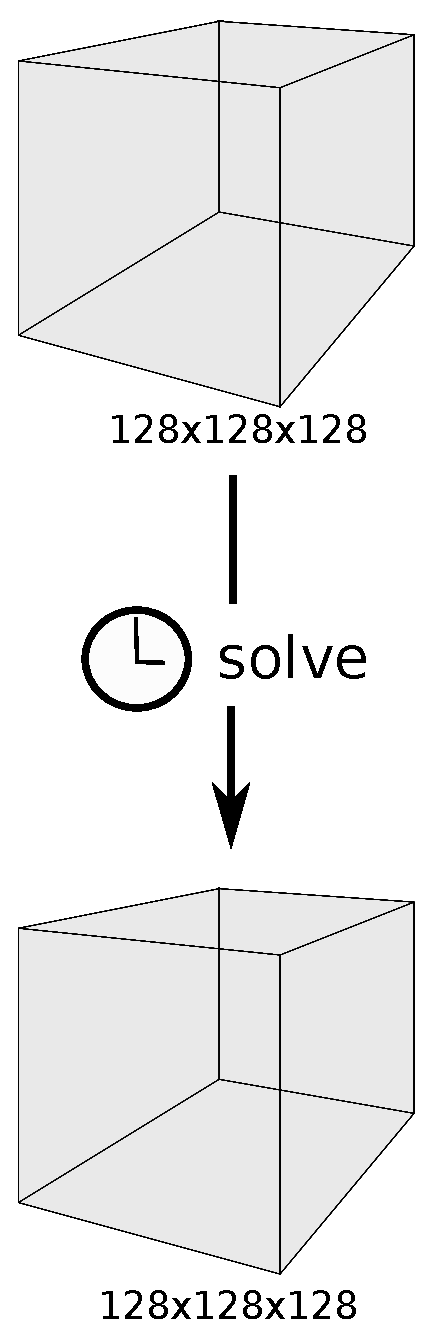
\includegraphics[scale=0.15]{img/classic_solver.eps} & 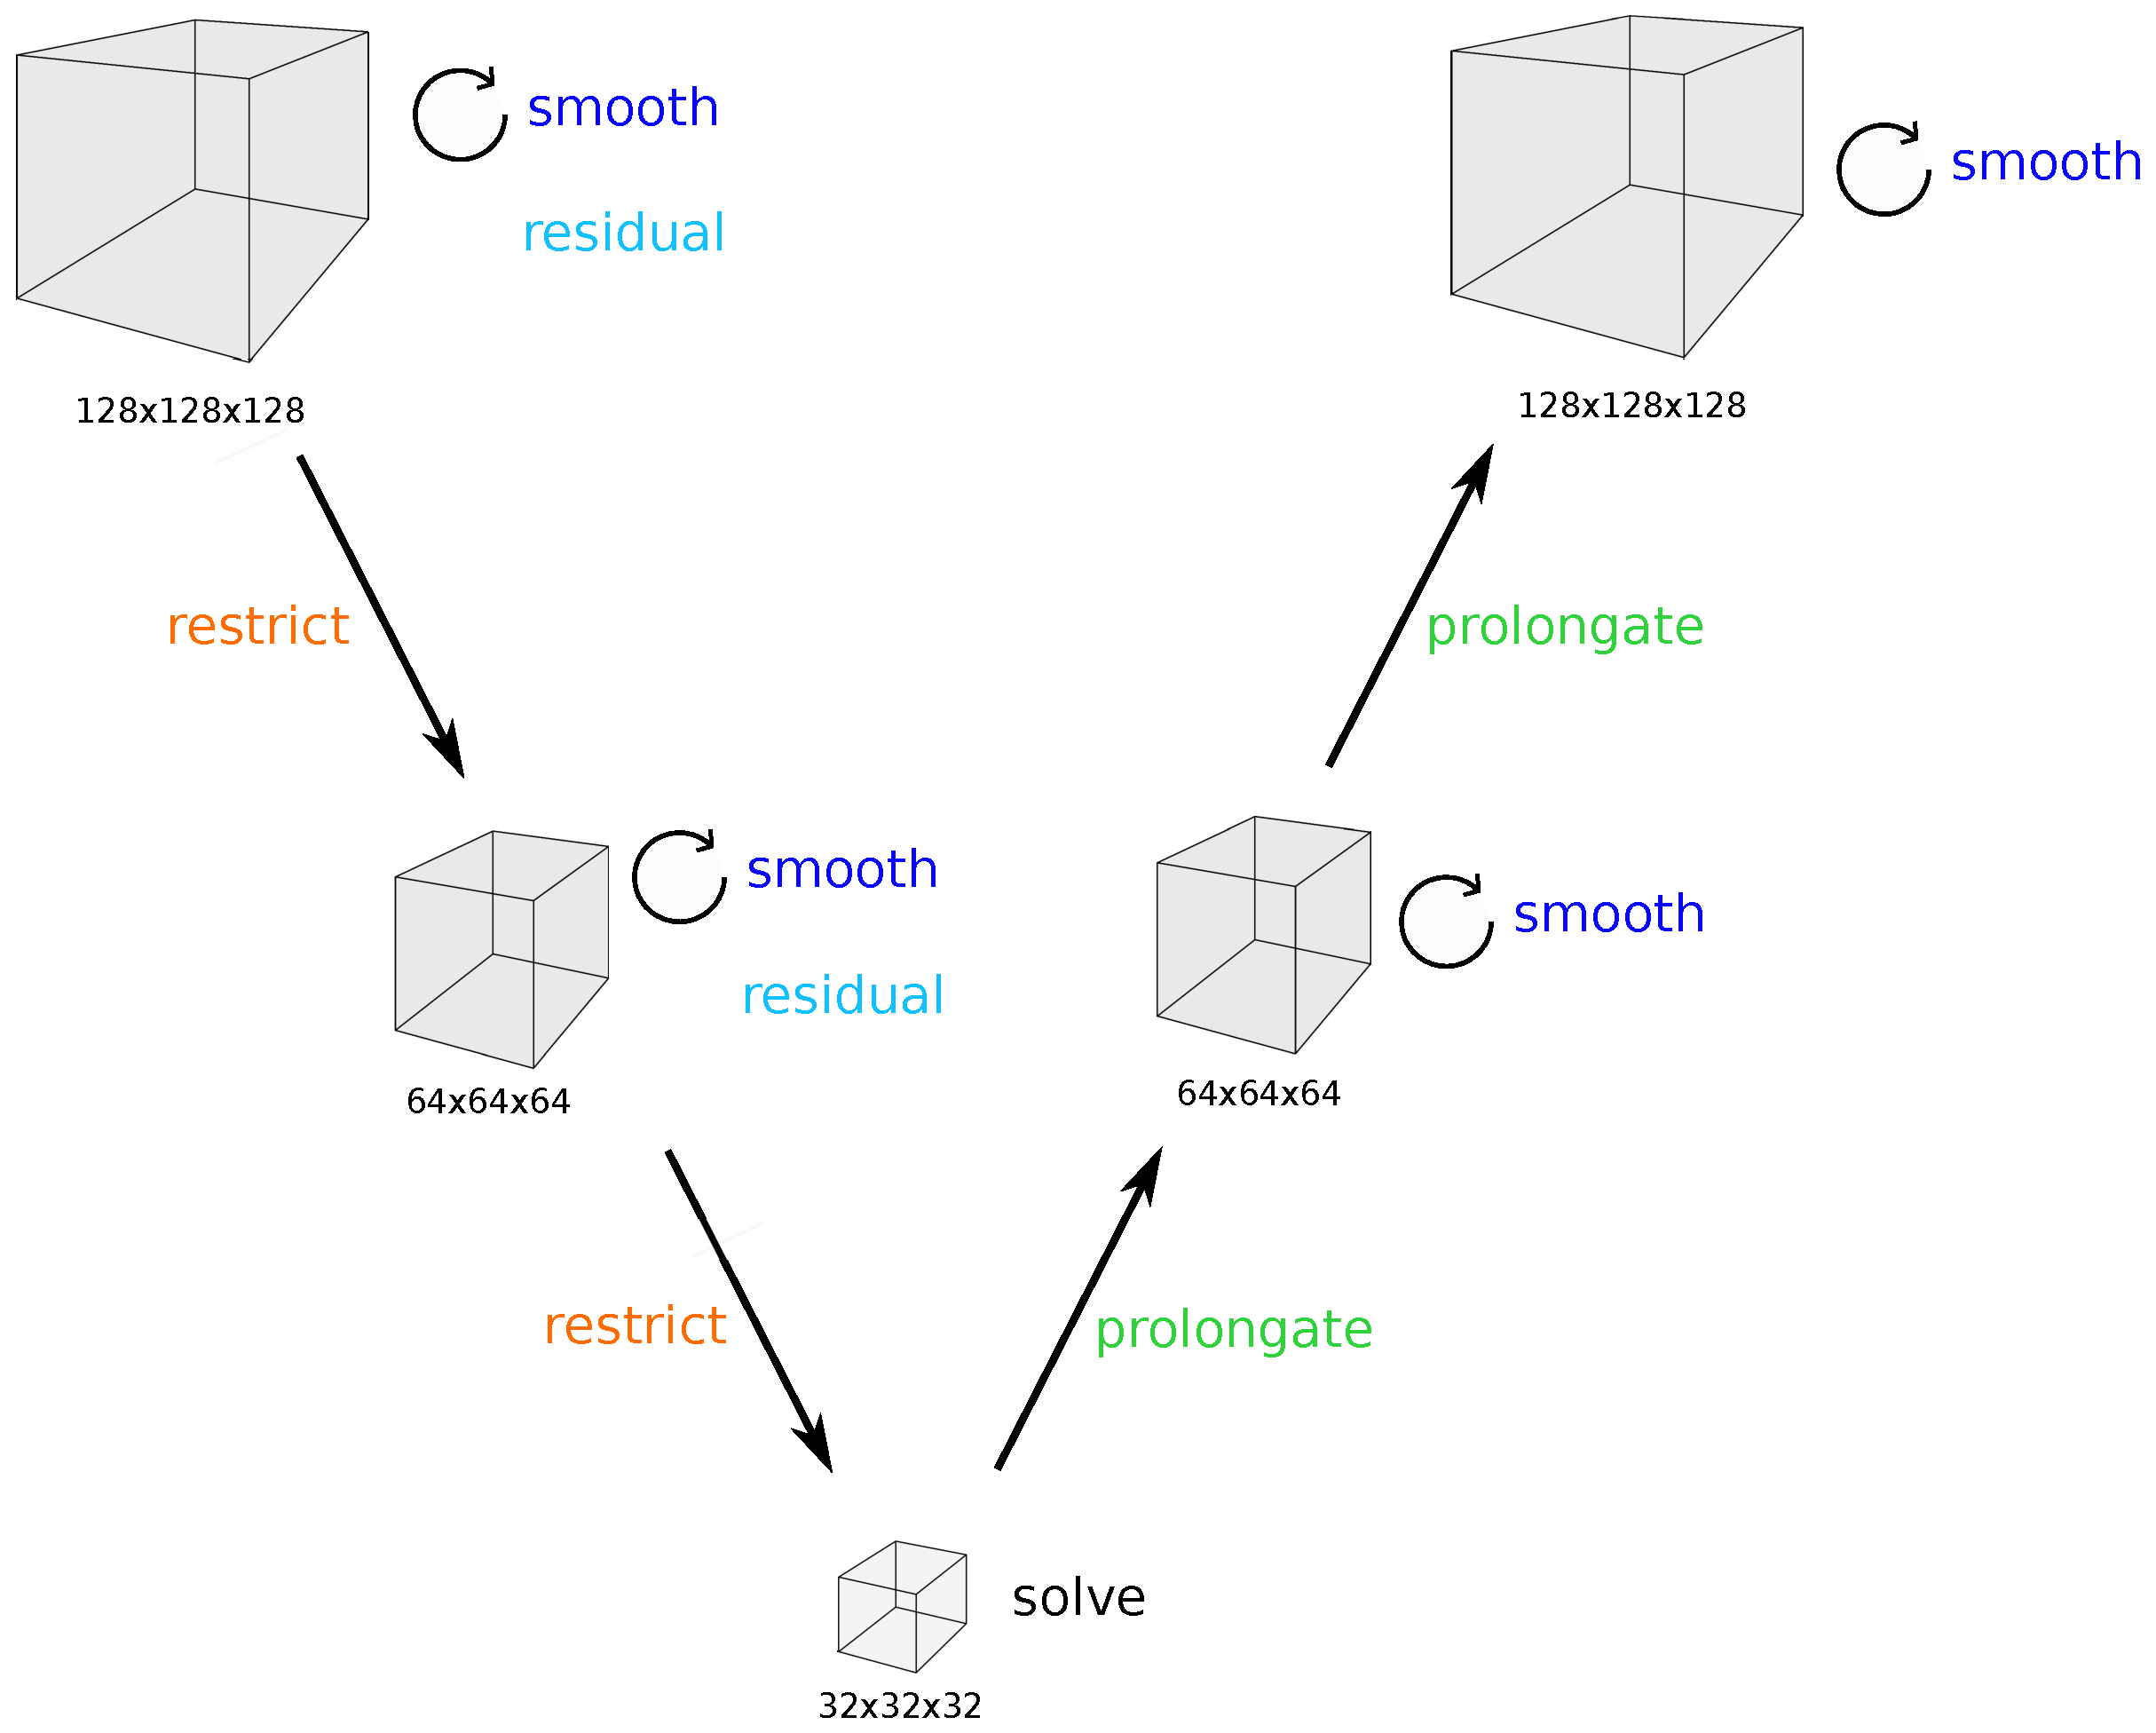
\includegraphics[scale=0.15]{img/multigrid.eps}  \\
		
	%\end{tabularx}
%	\includegraphics<1>[scale=0.25]{img/multigrid_scheme_smooth.png}
%	\includegraphics<2>[scale=0.25]{img/multigrid_scheme_all_labeled.png}
%	\includegraphics<3>[scale=0.25]{img/multigrid_scheme_brev.png}
%	\includegraphics<4>[scale=0.25]{img/multigrid_scheme_1.png}
\end{frame}

\begin{frame}{\Lift}

\begin{textblock*}{10cm}(0.75cm,2.5cm)
	\visible<2->{
	\begin{itemize}
		\small
		\item Generating high-performance programs from functional programming
		\item Optimizations encoded in rewrite-rules
	\end{itemize}
	}
	\vspace{0.3cm}
	\visible<3->{This Thesis:}
\end{textblock*}


\begin{textblock*}{10cm}(3cm,3.25cm)
	\includegraphics<2>[scale=0.175]{img/lift_gmg_workflow_0.eps}
	\includegraphics<3>[scale=0.175]{img/lift_gmg_workflow_1.eps}
	\includegraphics<4>[scale=0.175]{img/lift_gmg_workflow_2.eps}
	\includegraphics<5>[scale=0.175]{img/lift_gmg_workflow_3.eps}
	\includegraphics<6>[scale=0.175]{img/lift_gmg_workflow_4.eps}

\end{textblock*}

\end{frame}


\begin{frame}{Designing \Lift Expressions}
	\begin{textblock*}{10cm}(1cm,2.75cm)    
		\begin{itemize}
			\item<1-> Identifying the general structure of the operation
			\item<2-> Expressing the operation in 1 dimension
			\item<3-> Scaling the operation to 2 and 3 dimensions
		\end{itemize}		
	\end{textblock*}

	\begin{textblock*}{5cm}(1cm,5.5cm)    
		\includegraphics<2>[scale=0.28]{img/expressing_kernels_0.eps}
		\includegraphics<3>[scale=0.28]{img/expressing_kernels_1.eps}    
		\includegraphics<4>[scale=0.28]{img/expressing_kernels_2.eps}    
	\end{textblock*}

\end{frame}


\begin{frame}[fragile]{Smooth \& Residual}

	\begin{textblock*}{5cm}(1.25cm,4cm)    
		\includegraphics<1>[scale=0.45]{img/multiple_arrays_scheme_new_new.eps}
	\end{textblock*}
	
	\only<1-8>{
	\begin{textblock*}{5cm}(10cm,1.5cm)    
		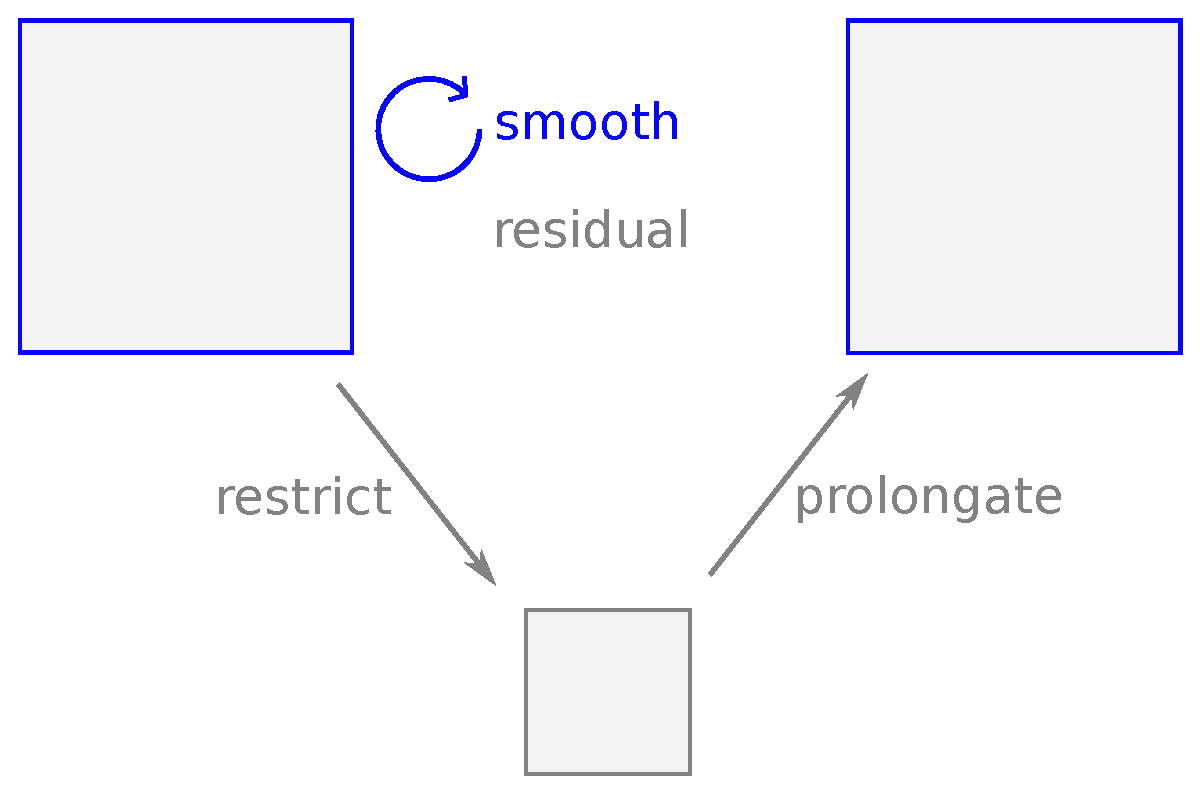
\includegraphics[scale=0.1]{img/indicator_0_smooth.eps}    
	\end{textblock*}
	}
	
	\only<9-9>{
	\begin{textblock*}{5cm}(10cm,1.5cm)    
		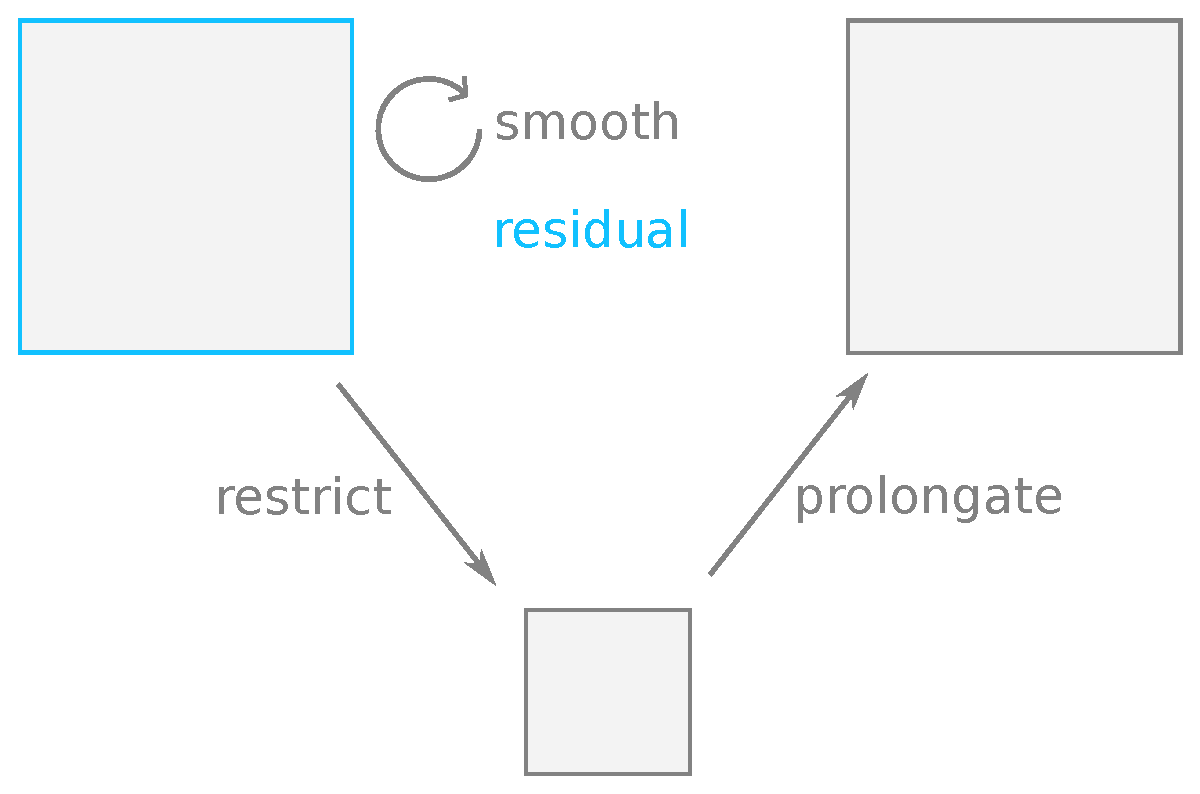
\includegraphics[scale=0.1]{img/indicator_0_residual.eps}    
	\end{textblock*}
	}
	
	\begin{textblock*}{10cm}(7.5cm,4.5cm)
		\tiny
%		\visible<5->{ \texttt{MapGlb(}} \visible<6->{ \\
%		 \hspace{0.5cm} \texttt{val a1  = tuple.get(0).at(0) }\\
%         \hspace{0.5cm} \texttt{val a2 = tuple.get(0).at(1)} \\
%         \hspace{0.5cm} \texttt{val a3 = tuple.get(0).at(2)} \\
%         \hspace{0.5cm} \texttt{val b1 = tuple.get(1).at(0)} \\
%         \hspace{0.5cm} \texttt{val b2 = tuple.get(1).at(1)} \\
%         \hspace{0.5cm} \texttt{val b3 = tuple.get(1).at(2)} \vspace{0.2cm}\\
%         }
         \visible<7->{
			\texttt{compute(Tuple t) = \{ } \\
		 	\hspace{0.5cm} \texttt{a1 = tuple<0>[0]}\\
         	\hspace{0.5cm} \texttt{a2 = tuple<0>[1]} \\
         	\hspace{0.5cm} \texttt{a3 = tuple<0>[2]} \\
         	\hspace{0.5cm} \texttt{b1 = tuple<1>[0]} \\
         	\hspace{0.5cm} \texttt{b2 = tuple<1>[1]} \\
         	\hspace{0.5cm} \texttt{b3 = tuple<1>[2]} \vspace{0.2cm}\\						
         }
         \only<2-6>{\vspace{0.25cm}}%oder einfach \\
		\only<7-8>{
		    \hspace{0.5cm} \texttt{\color{blue}smooth\color{black}(a1, a2, a3, b1, b2, b3)} \\
		}		 
		\only<9-9>{
		    \hspace{0.5cm} \texttt{\color{cyan}residual\color{black}(a1, a2, a3, b1, b2, b3)} \\
		}		
		
		\visible<7->{\}} \\
		
		\vspace{0.5cm}
		
		\visible<6->{\texttt{MapGlb( compute ) o}} \\
		\visible<5->{\texttt{Zip(}} \\
		\visible<4->{\hspace{0.5cm} \texttt{Slide(3,1) o}} \visible<3->{ \texttt{Pad(1,1,clamp) \$}} \visible<2->{\texttt{A,}} \\
		\visible<4->{\hspace{0.5cm} \texttt{Slide(3,1) o}} \visible<3->{ \texttt{Pad(1,1,clamp) \$}} \visible<2->{\texttt{B}} \visible<5->{ \hspace{0.0cm} \texttt{)}}
		\scriptsize

  		
%		\visible<5->{ MapGlb(} \visible<6->{ \\
%		 \hspace{0.5cm} val a1  = tuple.get(0).at(0) \\
%         \hspace{0.5cm} val a2 = tuple.get(0).at(1) \\
%         \hspace{0.5cm} val a3 = tuple.get(0).at(2) \\
%         \hspace{0.5cm} val b1 = tuple.get(1).at(0) \\
%         \hspace{0.5cm} val b2 = tuple.get(1).at(1) \\
%         \hspace{0.5cm} val b3 = tuple.get(1).at(2) \vspace{0.2cm}\\
%         }
%         \visible<7->{
%		 \hspace{0.5cm}  f(a1, a2, a3, b1, b2, b3)} \visible<5->{ \hspace{0.8cm})} \\
%		
%		%\visible<5->{)} \\
%		\visible<4->{Zip(} \\
%		\visible<3->{\hspace{0.5cm} Slide(3,1) o} \visible<2->{ Pad(1,1,clamp)} \visible<1->{A,} \\
%		\visible<3->{\hspace{0.5cm} Slide(3,1) o} \visible<2->{ Pad(1,1,clamp)} \visible<1->{B} \visible<4->{ \hspace{0.0cm} )}
%		
		
		
		
		
		
%		\begin{lstlisting}[mathescape=true]
%   	def f = "return a1 + a2 + a3 + b1 + b2 + b3;"
%    (A, B) => {
%        MapGlb(0)($\lambda$(tuple => {
%
%          val a1 = tuple._0.at(0)
%          val a2 = tuple._0.at(1)
%          val a3 = tuple._0.at(2)
%
%          val b1 = tuple._1.at(0)
%          val b2 = tuple._1.at(1)
%          val b3 = tuple._1.at(2)
%
%          f(a1, a2, a3, b1, b2, b3)
%
%        }) Zip(
%        Slide(3,1) o Pad(1,1,Pad.Boundary.Clamp)  A,
%        Slide(3,1) o Pad(1,1,Pad.Boundary.Clamp) B
%      )
%    })
% 
%		\end{lstlisting}
	\end{textblock*}

		
	\begin{textblock*}{10cm}(0.5cm, 2.5cm)
		\includegraphics[scale=0.35]<2>{img/residual1D_example_clearer_zip_bold_0.eps}
		\includegraphics[scale=0.35]<3>{img/residual1D_example_clearer_zip_bold_1.eps}
		\includegraphics[scale=0.35]<4>{img/residual1D_example_clearer_zip_bold_2.eps}
		\includegraphics[scale=0.35]<5>{img/residual1D_example_clearer_zip_bold_3.eps}
		\includegraphics[scale=0.35]<6>{img/residual1D_example_clearer_zip_bold_4.eps}
		\includegraphics[scale=0.35]<7>{img/residual1D_example_clearer_zip_bold_5.eps}
		\includegraphics[scale=0.35]<8>{img/residual1D_example_clearer_zip_bold_6.eps}
		\includegraphics[scale=0.35]<9->{img/residual1D_example_clearer_zip_bold_residual.eps} %This one should be residual specific

	\end{textblock*}
	
	
\end{frame}

%    def f = UserFun("f", Array("a1", "a2", "a3", "b1", "b2", "b3"),
%      "return a1 + a2 + a3 + b1 + b2 + b3;",
%      Seq(Float, Float, Float, Float, Float, Float), Float)
%
%    (A, B) => {
%
%        MapGlb(0)($\lambda$(tuple => {
%
%          val a1 = tuple._0.at(0)
%          val a2 = tuple._0.at(1)
%          val a3 = tuple._0.at(2)
%
%          val b1 = tuple._1.at(0)
%          val b2 = tuple._1.at(1)
%          val b3 = tuple._1.at(2)
%
%          toGlobal($\lambda$(x =>
%            f(a1, a2, a3, b1, b2, b3))) $\textdollar$ A
%
%        })) $\textdollar$ Zip(
%        Slide(3,1) o Pad(1,1,Pad.Boundary.Clamp) $\textdollar$ A,
%        Slide(3,1) o Pad(1,1,Pad.Boundary.Clamp) $\textdollar$ B
%      )
%    })


\begin{frame}{Restriction 1D}
	\begin{textblock*}{5cm}(10cm,1.5cm)    
		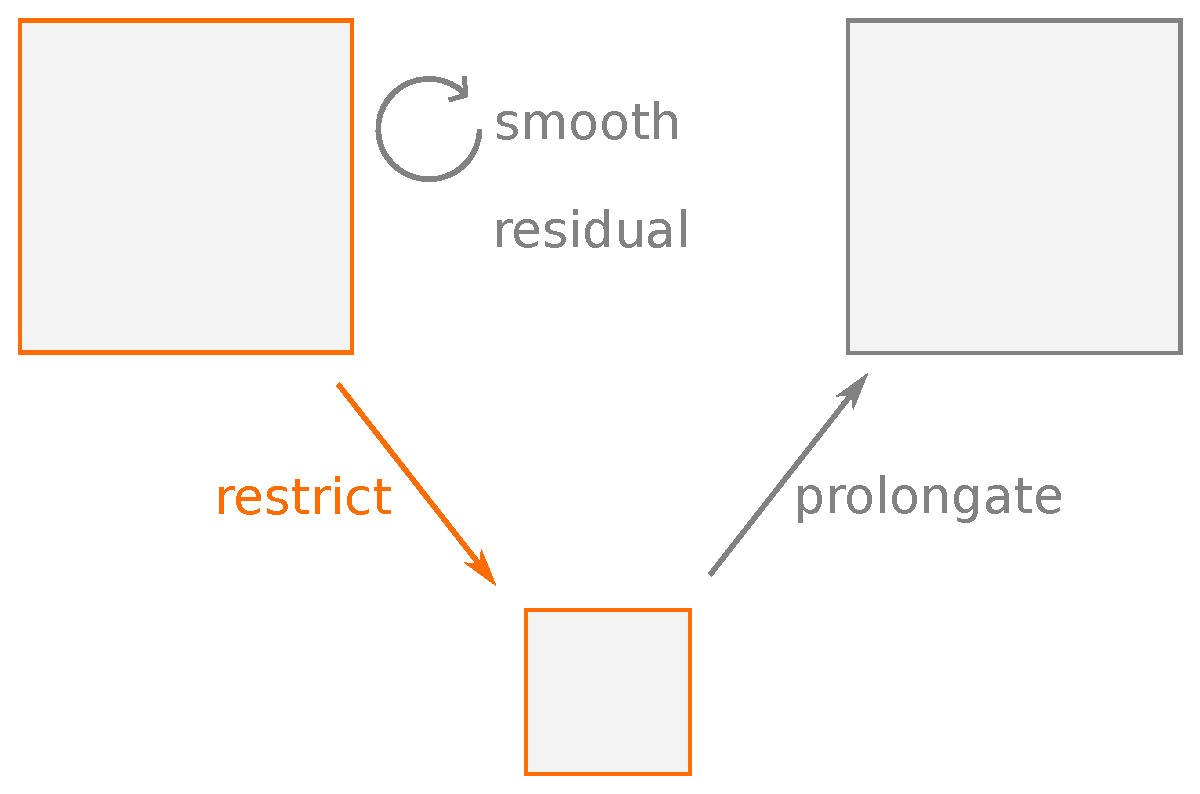
\includegraphics[scale=0.1]{img/indicator_1.eps}    
	\end{textblock*}
	
	\visible<1-1>{\includegraphics[scale=0.5]<1>{img/restriction1D_general_scheme.eps}}


	\begin{textblock*}{10cm}(0.75cm, 3cm)
		\includegraphics[scale=0.38]<2>{img/restriction1D_lift_scheme_smaller_bold_0.eps}
		\includegraphics[scale=0.38]<3>{img/restriction1D_lift_scheme_smaller_bold_1.eps}
		\includegraphics[scale=0.38]<4>{img/restriction1D_lift_scheme_smaller_bold_2.eps}
		\includegraphics[scale=0.38]<5>{img/restriction1D_lift_scheme_smaller_bold_3.eps}
	\end{textblock*}	
	
	\begin{textblock*}{10cm}(9cm,7.2cm)
		\scriptsize
		
		\visible<4->{\texttt{MapGlb(}} \\
		\visible<5->{\hspace{0.2cm} \texttt{Map($*\frac{1}{2}$) o} \\
		\hspace{0.2cm} \texttt{Reduce(+)}} \\ \visible<4->{\texttt{) o}} \\
		\visible<3->{\texttt{Split(2) \$}} \visible<2->{\texttt{ input}}
	\end{textblock*}
\end{frame}


\begin{frame}{Restriction 2D}
	\begin{textblock*}{5cm}(10cm,1.5cm)    
		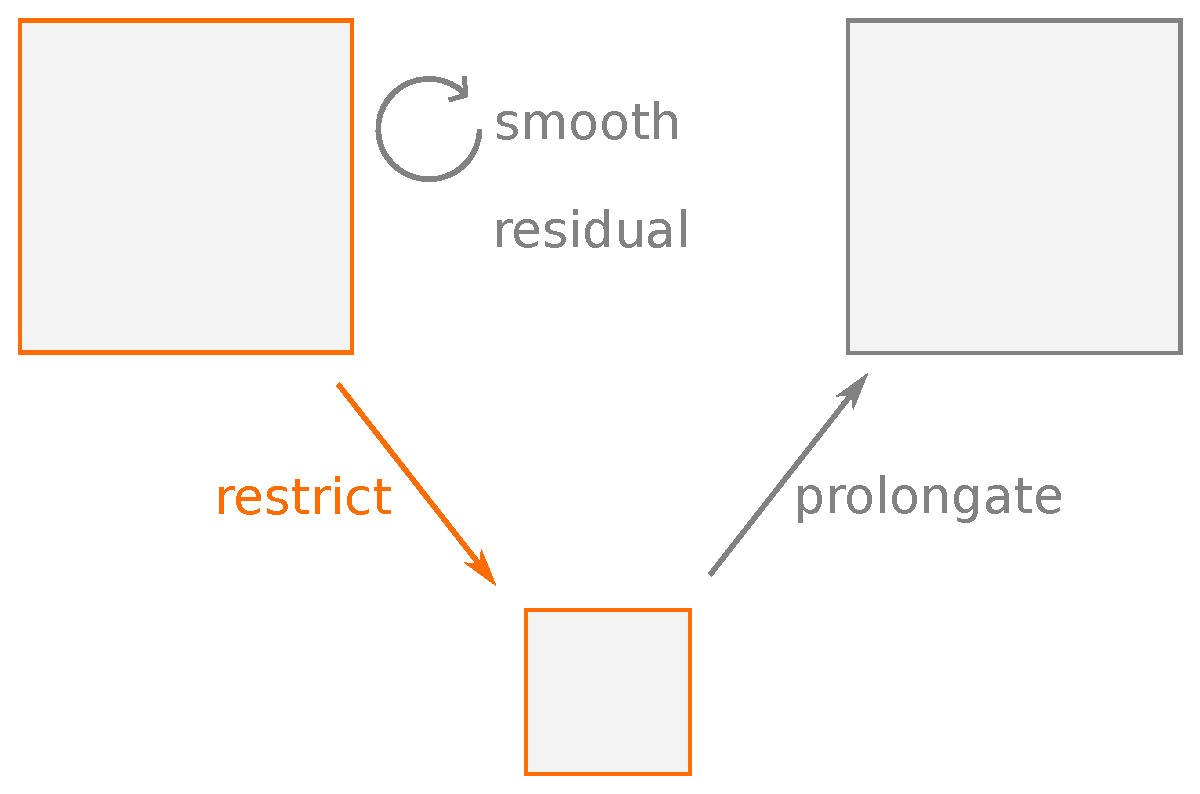
\includegraphics[scale=0.1]{img/indicator_1.eps}    
	\end{textblock*}
	\includegraphics[scale=0.4]<1>{img/restriction2D_lift_scheme_bold_0.eps}
	\includegraphics[scale=0.4]<2>{img/restriction2D_lift_scheme_bold_1.eps}
	\includegraphics[scale=0.4]<3>{img/restriction2D_lift_scheme_bold_2.eps}
	\includegraphics[scale=0.4]<4>{img/restriction2D_lift_scheme_bold_3.eps}
	\includegraphics[scale=0.4]<5>{img/restriction2D_lift_scheme_bold_4.eps}
	
	\begin{textblock*}{10cm}(8.75cm,6.5cm)
		\scriptsize
		
		\visible<3->{\texttt{MapGlb(} \\
		\hspace{0.2cm} \texttt{MapGlb(}} \\
		\visible<5->{\hspace{0.4cm} \texttt{Map($*\frac{1}{4}$) o} \\
		\hspace{0.4cm} \texttt{Reduce(+) o }}  \\
		\visible<4->{\hspace{0.4cm} \texttt{Join}}  \\ \visible<3->{\texttt{)) o }} \\
		\visible<2->{\textit{\texttt{Split2D(2)}} \$} \visible<1->{\texttt{ input}}
	\end{textblock*}
	
%	MapGlb(1)(
%MapGlb(0)(
%MapSeq(toGlobal(divideBy4)) o
%ReduceSeqUnroll(add, 0.0f) o
%Join()
%)
%) o Slide2D(2, 2)  input
\end{frame}


\begin{frame}{Prolongation}
	\begin{textblock*}{5cm}(10cm,1.5cm)    
		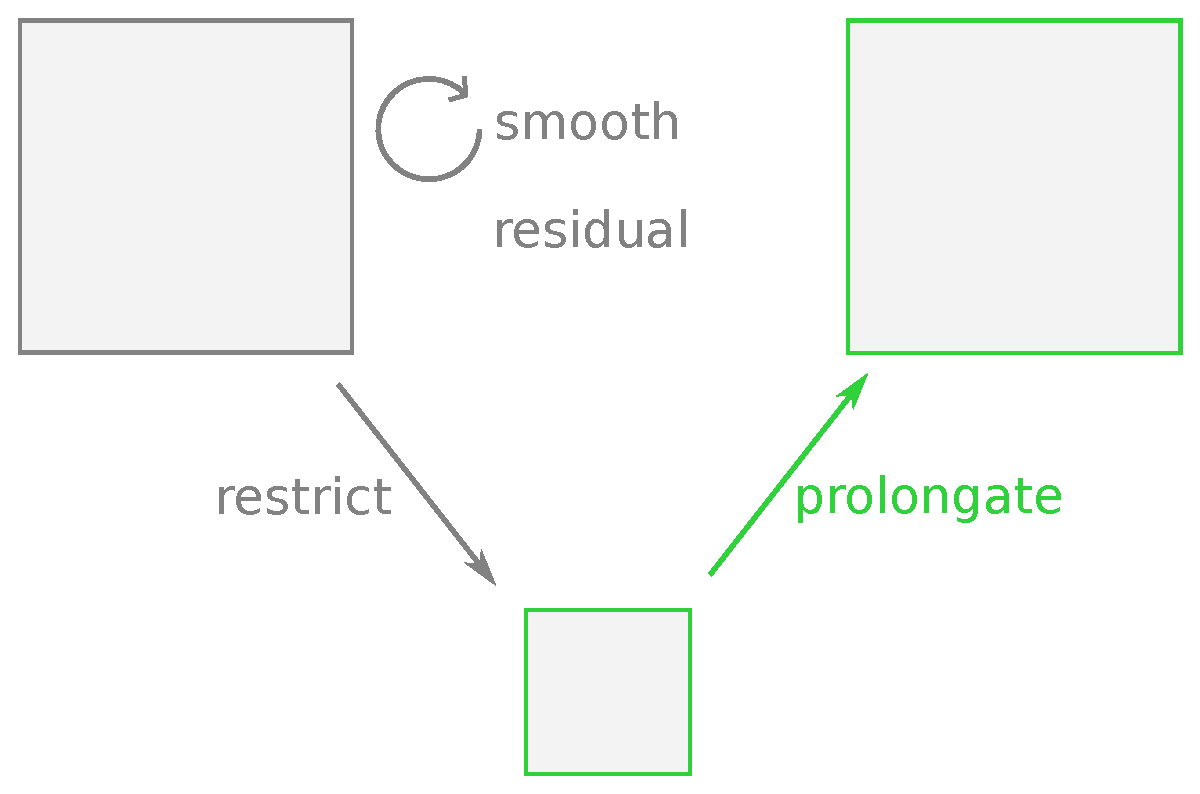
\includegraphics[scale=0.1]{img/indicator_2.eps}    
	\end{textblock*}
	\begin{center}
		\includegraphics[scale=0.58]<1>{img/prolongation1D_general_scheme_more.eps}
	\end{center}
	\includegraphics[scale=0.4]<2>{img/prolonation1D_MapPad_bold_0.eps}
	\includegraphics[scale=0.4]<3>{img/prolonation1D_MapPad_bold_1.eps}
	\includegraphics[scale=0.4]<4>{img/prolonation1D_MapPad_bold_2.eps}
	\includegraphics[scale=0.4]<5>{img/prolonation1D_MapPad_bold_3.eps}
	
	\begin{textblock*}{10cm}(8.5cm,7.5cm)
		\scriptsize
	
		\visible<5->{\texttt{Map(Pad(1,0,clamp)) o \\ Split(1) o}} \\
		\visible<4->{\texttt{Slide(2,1) o}} \\
		\visible<3->{\texttt{Pad(1,1,clamp) \$}} \visible<2->{\texttt{ input}}
	\end{textblock*}
\end{frame}

%(input, weights) =>
%//5
%MapGlb(0)(
%toGlobal(MapSeq(id)) o
%ReduceSeq(toGlobal(add), 0.0f) o
%toGlobal(MapSeq(\(tuple => mult(tuple._0, tuple._1))))
%) o
%//4
%Drop(1, 1) o
%Join() o
%//3
%Map(Map(\(tuple =>
%Zip(tuple._0, tuple._1)
%))) o
%Map(\(nbh =>
%Zip(nbh,
%Split(2) o Pad(2,0,Mirror) $ weights)
%)) o
%//2
%Map(Pad(1,0,Wrap)) o Split(1) o
%//1
%Slide(2,1) o
%Pad(1,1,Pad.Boundary.Clamp)
%$ input

\begin{frame}{Prolongation}
	\begin{textblock*}{5cm}(10cm,1.5cm)    
		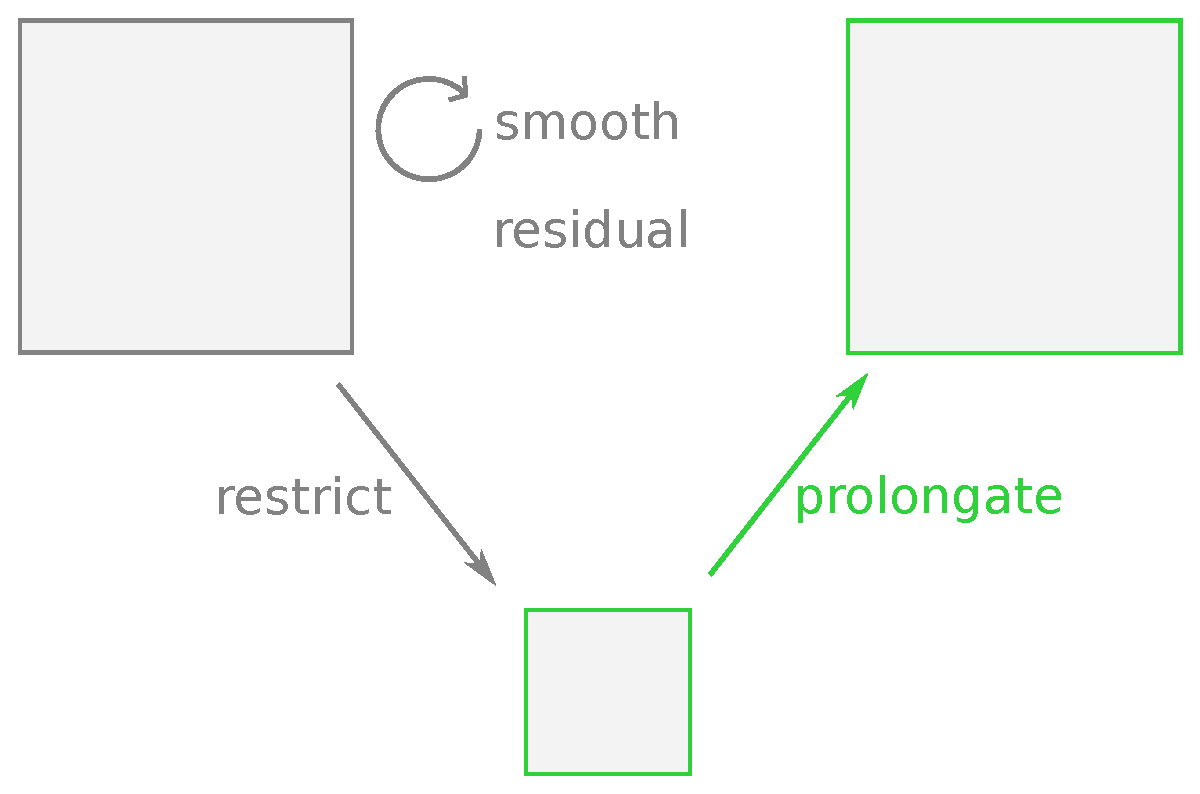
\includegraphics[scale=0.1]{img/indicator_2.eps}    
	\end{textblock*}
	
	\begin{textblock*}{10cm}(0.75cm, 2cm)
		\includegraphics[scale=0.44]<1>{img/prolonation1D_zip_weights_extended_bold_0.eps}
		\includegraphics[scale=0.44]<2>{img/prolonation1D_zip_weights_extended_bold_1.eps}
		\includegraphics[scale=0.44]<3>{img/prolonation1D_zip_weights_extended_bold_2.eps}
		\includegraphics[scale=0.44]<4>{img/prolonation1D_zip_weights_extended_bold_3.eps}
		\includegraphics[scale=0.44]<5>{img/prolonation1D_zip_weights_extended_bold_4.eps}
		\includegraphics[scale=0.44]<6>{img/prolonation1D_zip_weights_extended_bold_5.eps}
		\includegraphics[scale=0.44]<7->{img/prolonation1D_zip_weights_extended_bold_6.eps}		
	\end{textblock*}
		
	\begin{textblock*}{10cm}(7.5cm,4.5cm)
		\tiny
		
		\visible<7->{\texttt{Map(Map(tuple =>}} \\
		\hspace{0.5cm} \visible<7->{\texttt{Zip(}} \\
		\hspace{1cm} \visible<7->{\texttt{tuple<0>,}} \\
		\hspace{1cm} \visible<7->{\texttt{tuple<1>}} \\
		\hspace{0.5cm} \visible<7->{\texttt{)}} \\
		\visible<7->{\texttt{)) o}}
		
		\visible<2->{\texttt{Map(nbh =>}} \\
		\hspace{0.5cm} \visible<6->{\texttt{Zip(}} \\
		\hspace{1cm} \visible<2->{\texttt{nbh,}} \\
		\hspace{1cm} \visible<5->{\texttt{Split(2) o }}
		\visible<4->{\texttt{Pad(2,0,Mirror) \$ }} \\
		\hspace{1cm} \visible<3->{\texttt{weights}} \\
		\hspace{0.5cm} \visible<6->{\texttt{)}} \\
		\visible<2->{\texttt{) o}}
	\end{textblock*}
	
	\begin{textblock*}{10cm}(7.5cm,7.75cm)
		\tiny
	\color{black!35}
		\visible<1->{\texttt{Map(Pad(1,0,wrap)) o \\ Split(1) o}} \\
		\visible<1->{\texttt{Slide(2,1) o}} \\
		\visible<1->{\texttt{Pad(1,1,clamp) \$}} \visible<1->{\texttt{ input}}
	\end{textblock*}
	\color{black}
\end{frame}

\begin{frame}{Prolongation}
	\begin{textblock*}{5cm}(10cm,1.5cm)    
		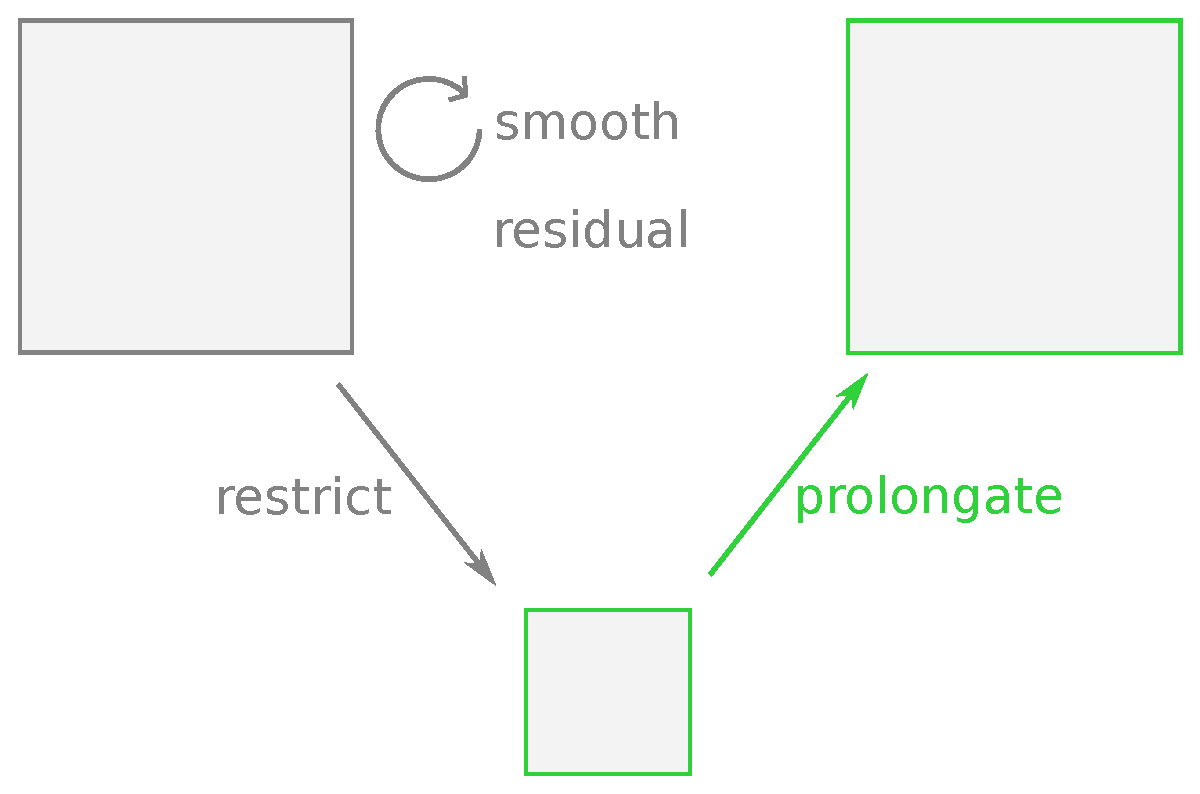
\includegraphics[scale=0.1]{img/indicator_2.eps}    
	\end{textblock*}
	
	\begin{center}
		\includegraphics[scale=0.58]<1>{img/prolongation1D_general_scheme_more.eps}
	\end{center}		
	
	\begin{textblock*}{10cm}(0.75cm, 3.5cm)
	\includegraphics[scale=0.45]<2>{img/prolonation1D_Drop_full_structure_bold_0.eps}
	\includegraphics[scale=0.45]<3->{img/prolonation1D_Drop_full_structure_bold_1.eps}
	\end{textblock*}

	\begin{textblock*}{10cm}(0.75cm, 7cm)
		\scriptsize
		\begin{itemize}
			\item<4-> \texttt{Drop(l,r)} was introduced in this thesis
			\item<4-> Extends \Lift to be capable of expressing prolongation
		\end{itemize}
	\end{textblock*}

	
	\begin{textblock*}{10cm}(9cm,6.7cm)
		\tiny
		
		\visible<3->{\texttt{Drop(1,1) o}} \\
		\color{black!35}
		\visible<2->{\texttt{Map(Map(tuple =>}} \\
		\hspace{0.5cm} \visible<2->{\texttt{Zip(}} \\
		\hspace{1cm} \visible<2->{\texttt{tuple<0>,}} \\
		\hspace{1cm} \visible<2->{\texttt{tuple<1>)}} \\
		\hspace{0.5cm} \visible<2->{\texttt{)}} \\
		\visible<2->{\texttt{)) o}}
		
		\visible<2->{\texttt{[...]}}
		\color{black}
	\end{textblock*}

\end{frame}

\begin{frame}{Prolongation}
	\begin{textblock*}{5cm}(10cm,1.5cm)    
		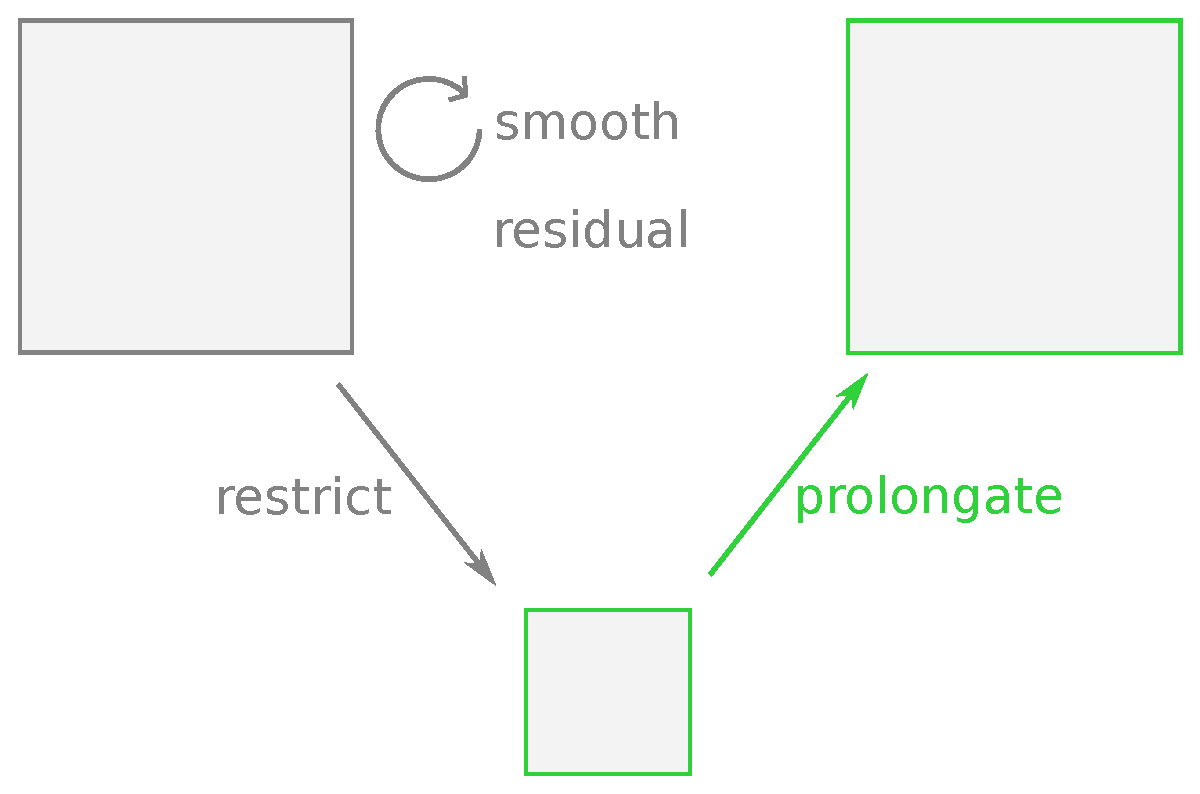
\includegraphics[scale=0.1]{img/indicator_2.eps}    
	\end{textblock*}
	
	\begin{textblock*}{10cm}(0.75cm, 3cm)
	\includegraphics[scale=0.45]<1>{img/prolonation1D_computation_bold_0.eps}
	\includegraphics[scale=0.45]<2>{img/prolonation1D_computation_bold_1.eps}
	\includegraphics[scale=0.45]<3>{img/prolonation1D_computation_bold_2.eps}
	\includegraphics[scale=0.45]<4>{img/prolonation1D_computation_bold_3.eps}
	\end{textblock*}

	\begin{textblock*}{10cm}(7.25cm,6.75cm)
		\tiny
		\color{black}
		\visible<2->{\texttt{MapGlb(}} \\
		\hspace{0.5cm}\visible<4->{\texttt{Reduce(+) o}} \\
		\hspace{0.5cm}\visible<3->{\texttt{MapSeq(}} \\
		\hspace{1cm}\visible<3->{\texttt{tuple<0> * tuple<1>\\
		\hspace{0.5cm}) }} \\
		\visible<2->{\texttt{) o}} \\
		
		\color{black!35}
		\visible<1->{\texttt{Drop(1,1) o}} \\
		\color{black}
%		\visible<1->{\texttt{Map(Map(tuple =>}} \\
%		\hspace{0.5cm} \visible<1->{\texttt{Zip(}} \\
%		\hspace{1cm} \visible<1->{\texttt{tuple.get(0),}} \\
%		\hspace{1cm} \visible<1->{\texttt{tuple.get(1)}} \\
%		\hspace{0.5cm} \visible<1->{\texttt{)}} \\
%		\visible<1->{\texttt{)) o}}
		\visible<1->{\texttt{[...]}}
	\end{textblock*}

\end{frame}

\begin{frame}{Evaluation}
\scriptsize

	\visible<1->{
	
		\begin{itemize}
			\item<1-> \Lift does not support building entire programs yet 
			\item<1-> All operations expressed in \Lift in multiple dimensions
		\end{itemize}
	}
	\vspace{0.3cm}
	\visible<2->{
		Performance comparison of individual operations 
		\begin{itemize}
			\item OpenCL kernels generated from handwritten \Lift low-level expressions 
			\item OpenCL kernels generated with the Polyhedral Parallel Code Generation (PPCG) compiler 
		\end{itemize}
		
		\visible<3->{
		\vspace{0.3cm}
		Workflow
		\begin{itemize}
			\item Used GPU: Nvidia GeForce GTX 1080
			\item All parameters auto-tuned with the Auto Tuning Framework (ATF)
			\item Tuning time: 1 hour per framework per operation per input size
		\end{itemize}
		}	
	}
\end{frame}


\begin{frame}{Runtime Comparison}
	\only<1>{
		\begin{textblock*}{10cm}(1.5cm,2.15cm)
			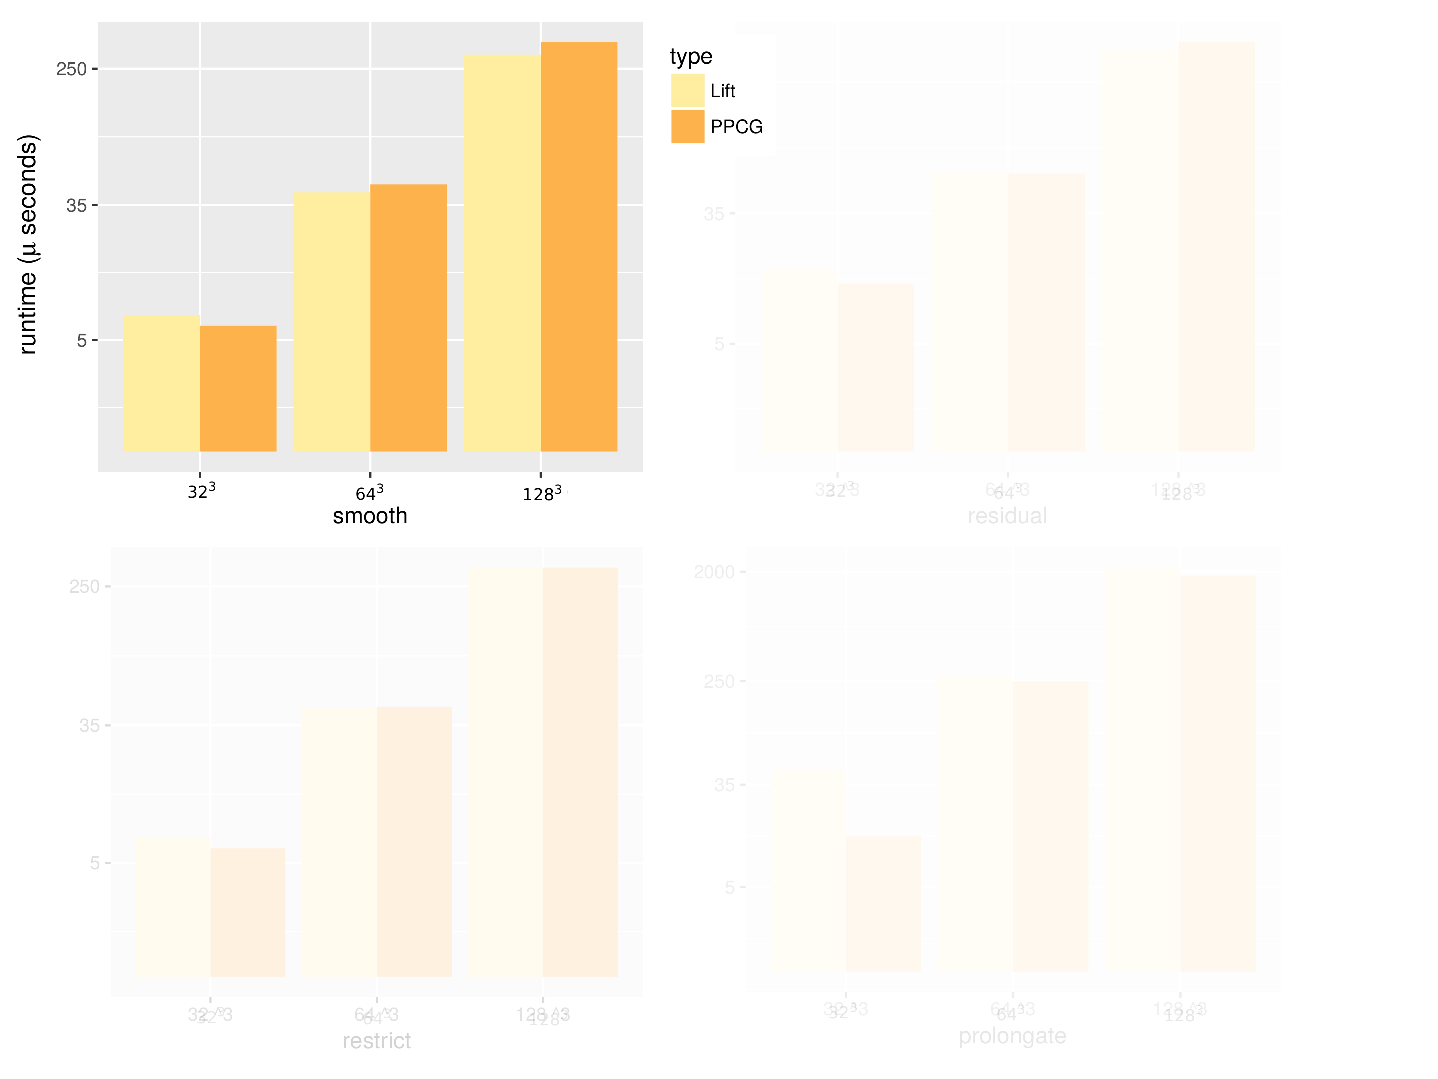
\includegraphics[scale=0.375]{img/plots/runtime_4_edited_transparent.eps}
		\end{textblock*}
	}

	\only<1>{
		\begin{textblock*}{10cm}(6cm,3cm)
			\small
			\begin{itemize}
				\item x: output elements ($32^3$, $64^3$, $128^3$)
				\item y: runtime in $\mu s$ (lower is better)
			\end{itemize}
		\end{textblock*}	
	}	
	
	\only<1>{
		\begin{textblock*}{10cm}(0cm,5.75cm)
			\small
			\color{yellow} \colorbox{black!20}{\hspace{2.4cm} \Lift \hspace{1cm} \color{orange} PPCG} \color{black}
		\end{textblock*}	
	}		
	
	\only<2->{
		
		\begin{textblock*}{10cm}(1.5cm,2.15cm)
			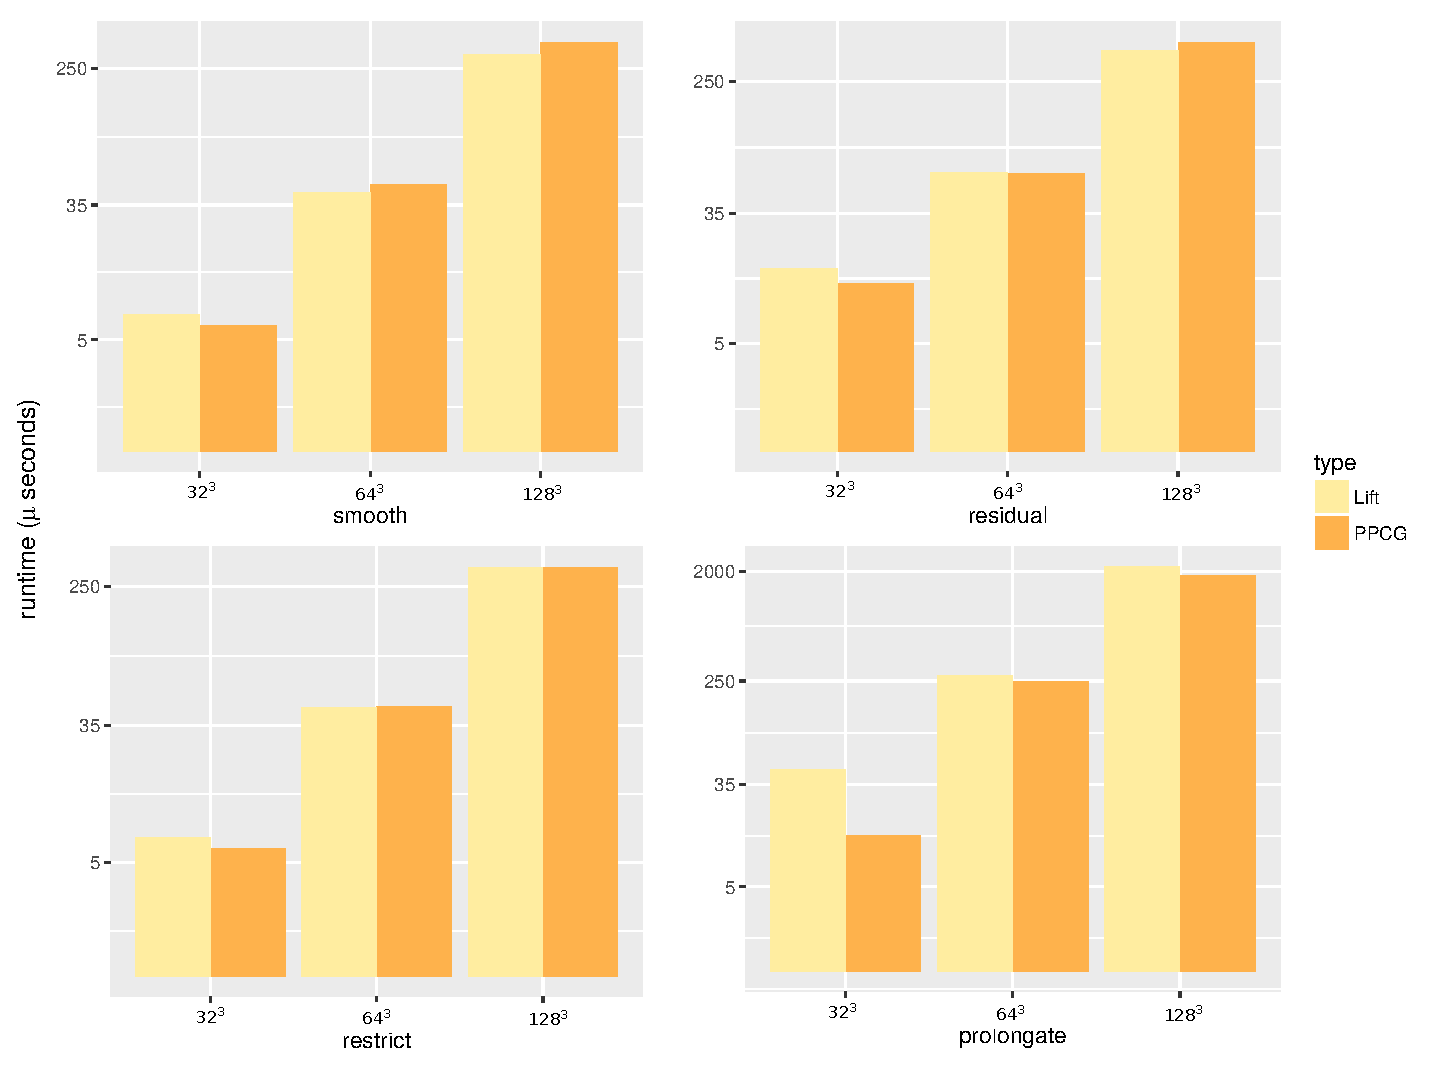
\includegraphics[scale=0.375]{img/plots/runtime_4_edited.eps}
		\end{textblock*}
	}
\end{frame}


\begin{frame}{Speedup Comparison}
	\only<1>{
		\begin{textblock*}{10cm}(2.5cm,2.5cm)
		%\begin{center}
			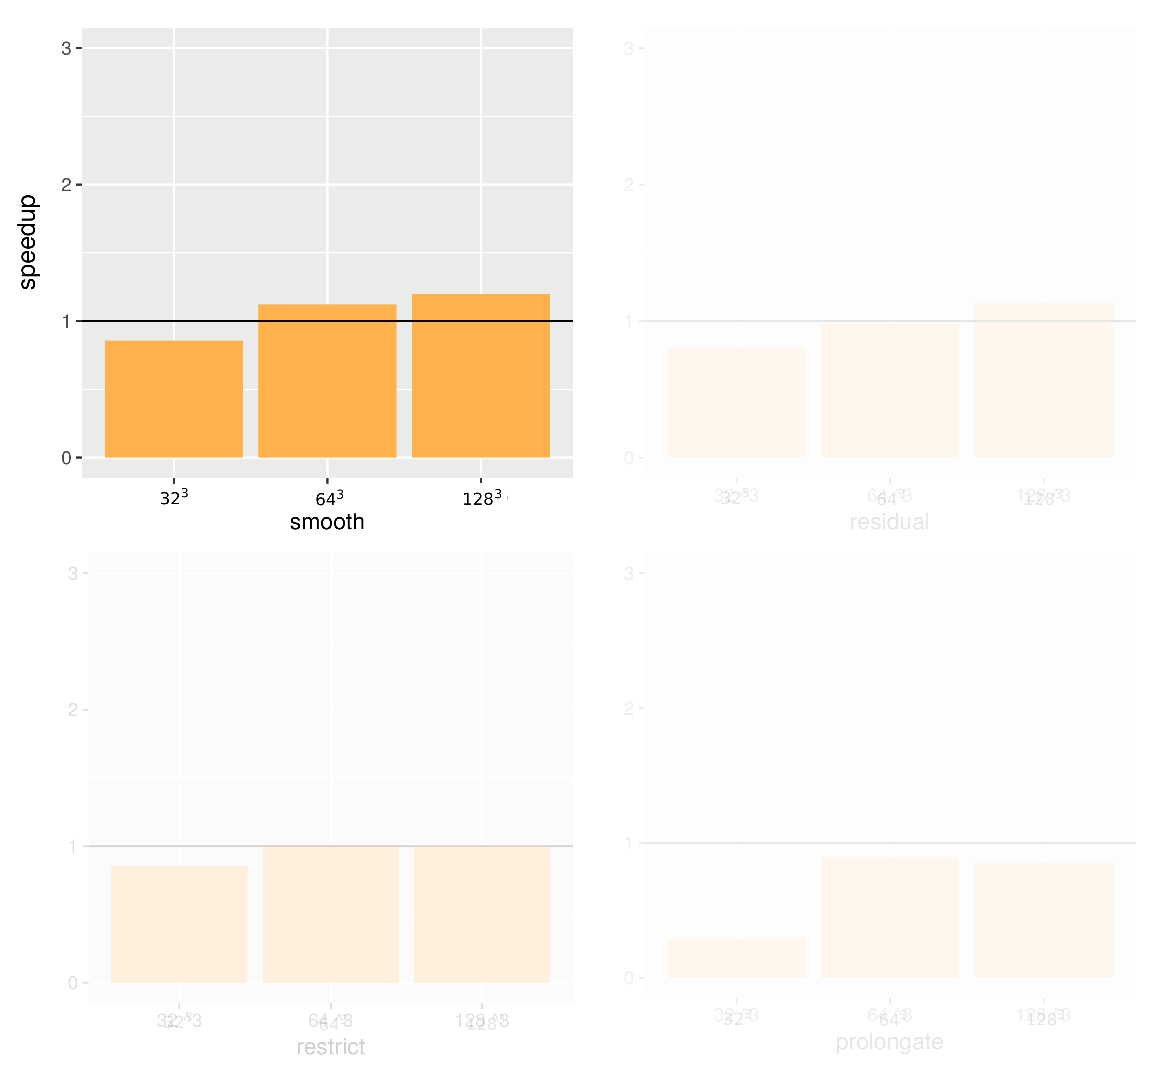
\includegraphics[scale=0.35]{img/plots/speedup_4_edited_transparent.eps}
		%\end{center}
		\end{textblock*}
	}
	
	\only<1>{
		\begin{textblock*}{10cm}(6cm,3cm)
			\small
			\begin{itemize}
				\item x: output elements ($32^3$, $64^3$, $128^3$)
				\item y: speedup (higher is better)
			\end{itemize}
		\end{textblock*}	
	}	
	
	\only<2->{
	\begin{textblock*}{10cm}(2.5cm,2.5cm)
	%\begin{center}
		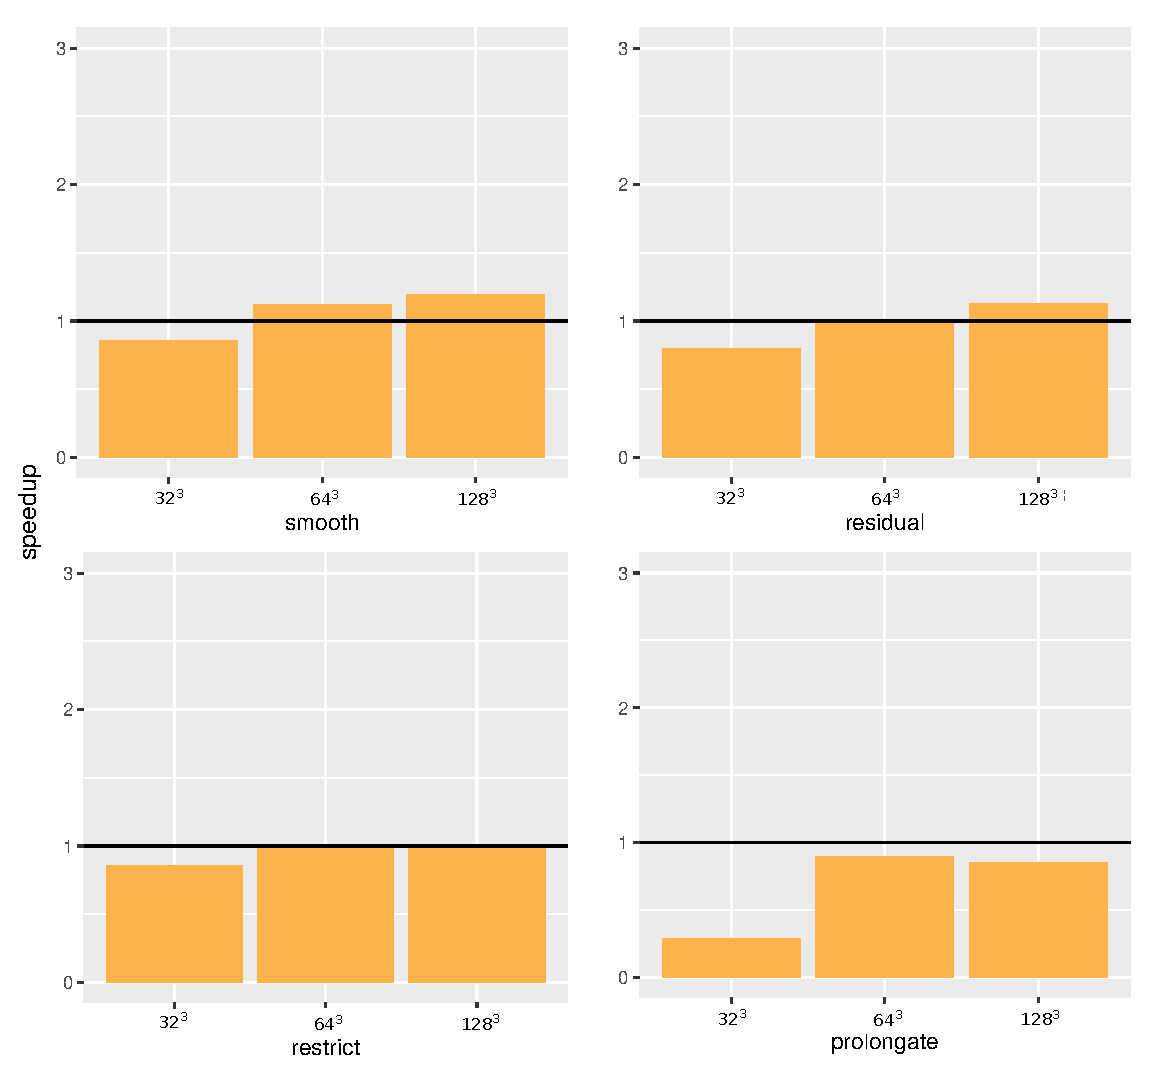
\includegraphics[scale=0.35]{img/plots/speedup_4_edited.eps}
	%\end{center}
	\end{textblock*}
	}
	
\end{frame}


\begin{frame}{GMG Program}
	\scriptsize
	%was ist hier los? Warum tut \only das, was eigentlich \visible tun sollte?
	
	\only<1->{
	\begin{textblock*}{10cm}(1.25cm,2.5cm)
		In a GMG solver the operations vary in number of execution, so further evaluation was necessary:
	\end{textblock*}
	}
	
	\only<2->{
	\begin{textblock*}{10cm}(2.5cm,3.25cm)
		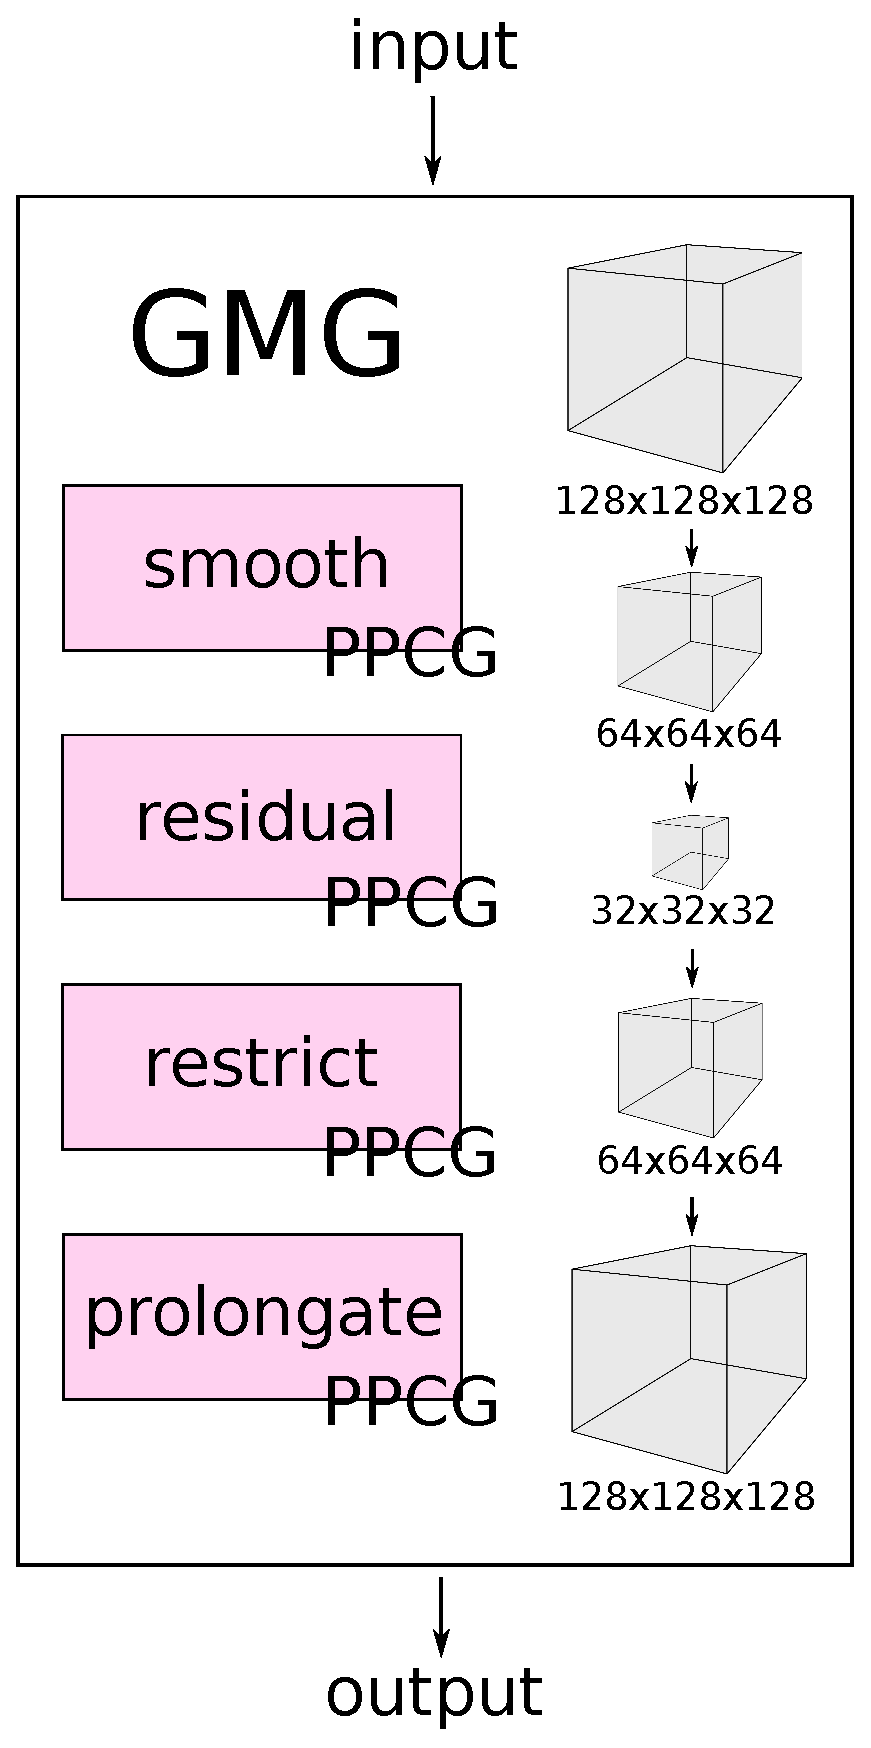
\includegraphics[scale=0.175]{img/gmg_program_ppcg.eps}
	\end{textblock*}
	}

	\only<3->{	
	\begin{textblock*}{10cm}(6cm,3.25cm)
		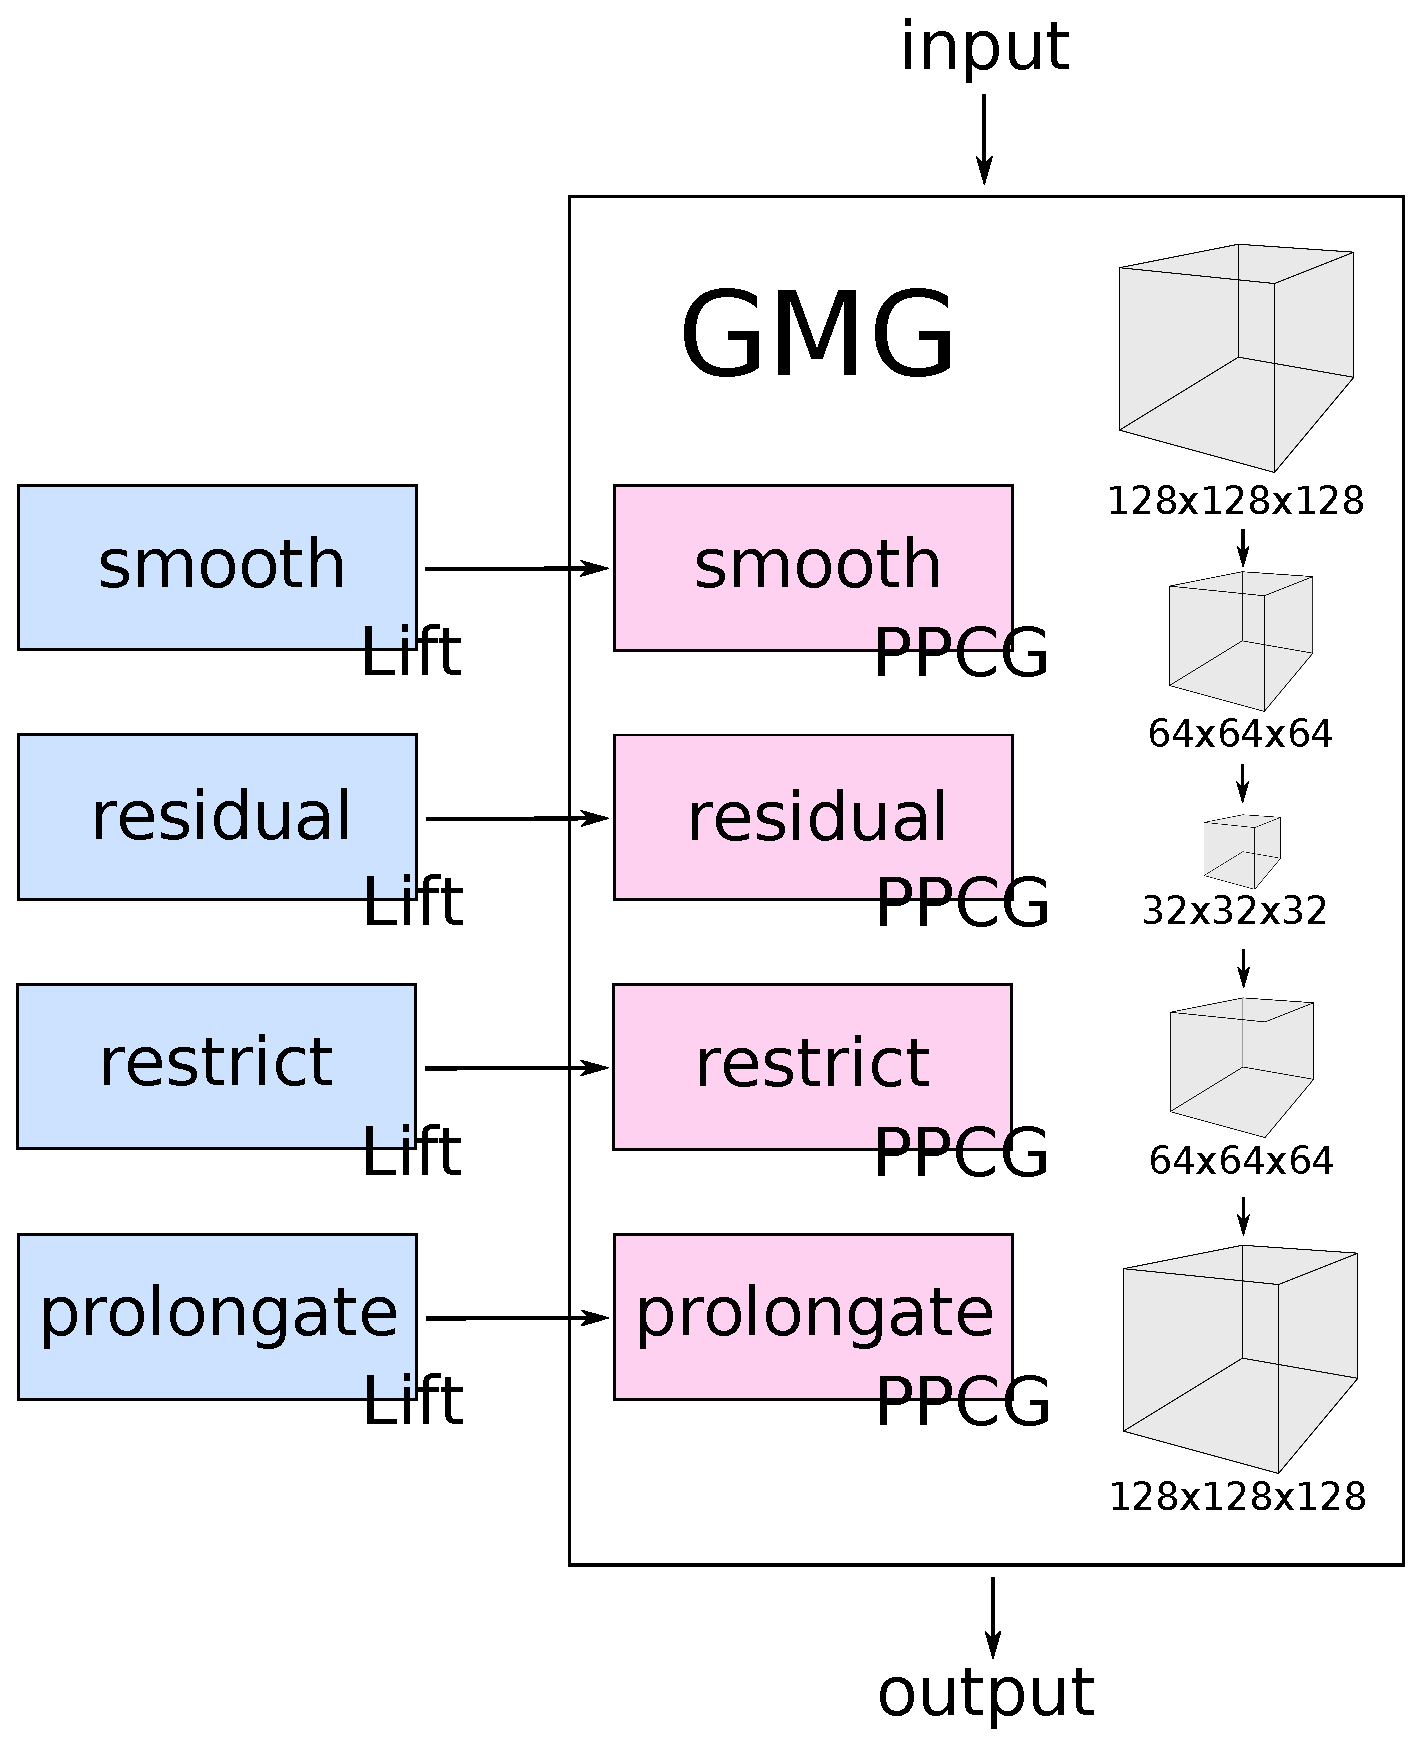
\includegraphics[scale=0.175]{img/gmg_program_lift.eps}
	\end{textblock*}
	}

	\only<5->{	
	\begin{textblock*}{10cm}(1.5cm,3.85cm)
		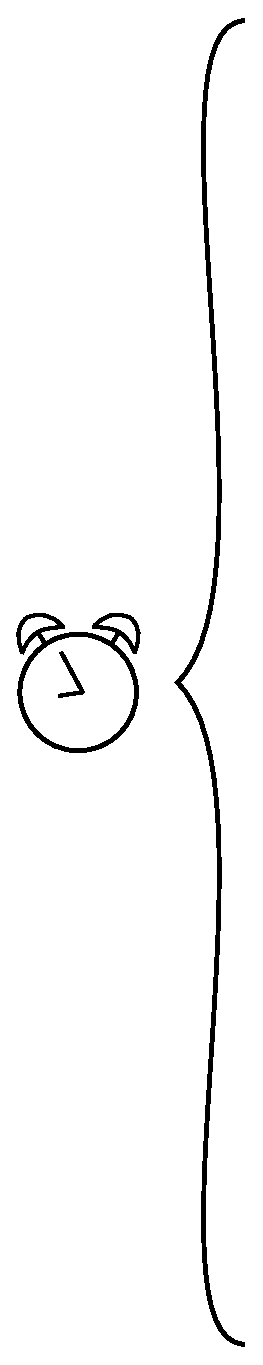
\includegraphics[scale=0.175]{img/program_measure.eps}
	\end{textblock*}
	}

	\only<4->{
	\begin{textblock*}{10cm}(1.25cm,8.5cm)
		For each operation the best parameters from the previous auto-tuning are used	
	\end{textblock*}
	}
\end{frame}



\begin{frame}{GMG Program Runtime Comparison}

	\begin{textblock*}{10cm}(0.25cm,3.5cm)
		\scriptsize
		\begin{itemize}
			\item<1-> Residual, restrict, prolongate each\\ executed 2 times
			\item<1-> Smooth executed 24 times
			\vspace{0.5cm}
			\item<3-> Small improvement in smooth has \\ large impact on overall runtime
			\item<4-> Experiments with optimizations \\ for iterative kernels in \Lift
		\end{itemize}
	\end{textblock*}
	
	\only<2->{
		\begin{textblock*}{10cm}(5.5cm,2.5cm)
			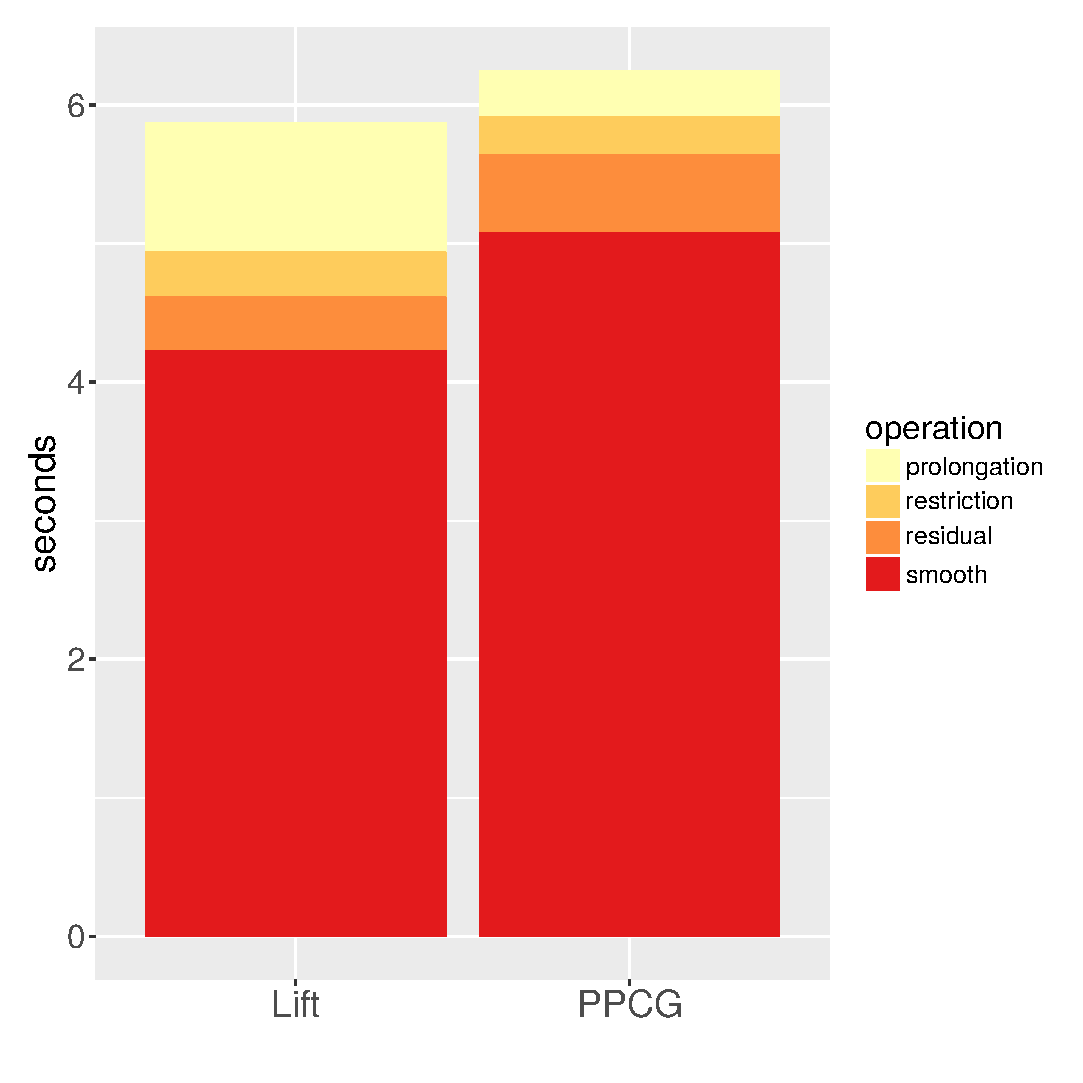
\includegraphics[scale=0.35]{img/plots/v_cycle_edited.eps}
		\end{textblock*}
	}
		
\end{frame}

\begin{frame}
\Large
\center
Questions?

\end{frame}





\begin{frame}{Backup Slides}

\end{frame}

\begin{frame}{Error Smoothing}
	\center
	\includegraphics[scale=0.275]<1>{img/errorSmoothing_0.png}
	\includegraphics[scale=0.275]<2>{img/errorSmoothing_1.png}
	\includegraphics[scale=0.275]<3>{img/errorSmoothing.png}
\end{frame}

\begin{frame}{Smooth}
	\center
	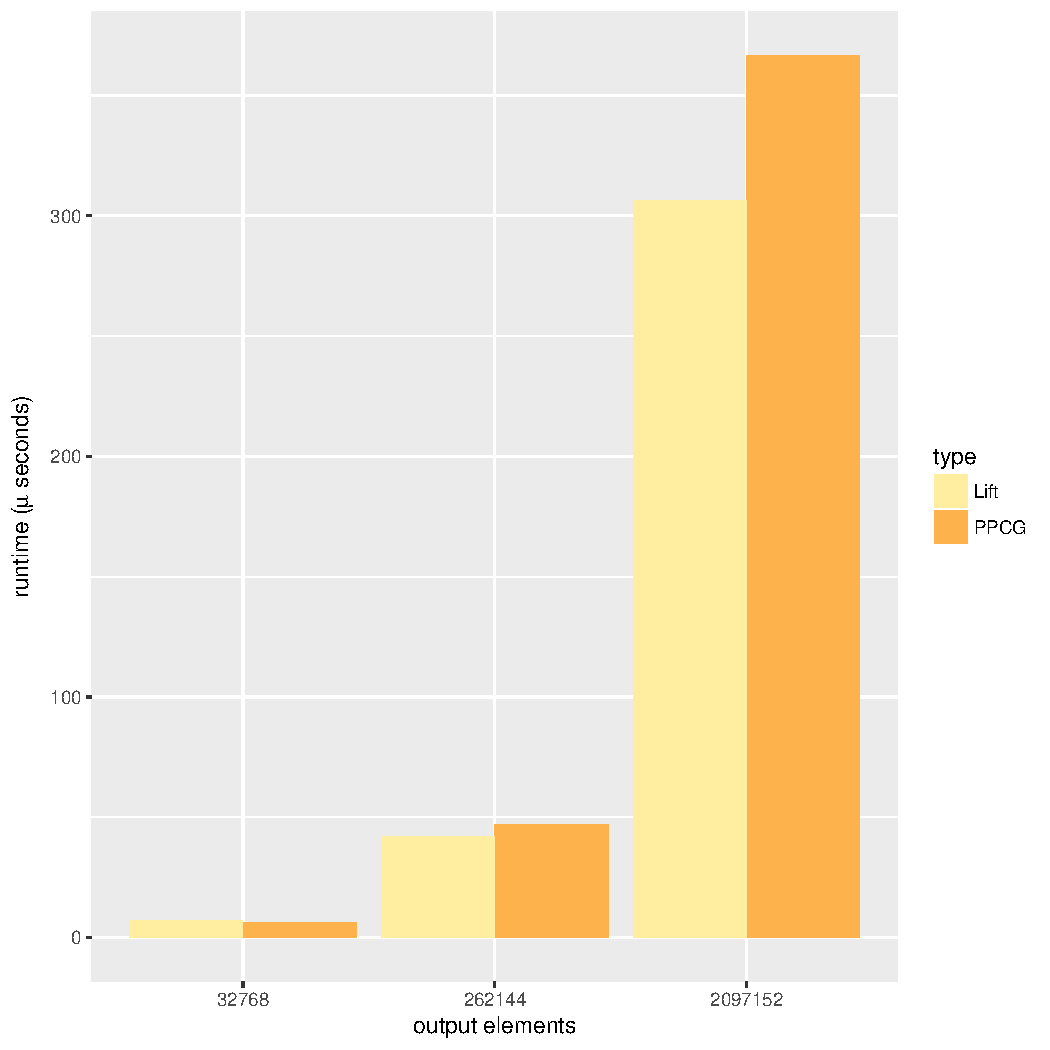
\includegraphics[scale=0.35]{img/plots/smooth.pdf}
\end{frame}

\begin{frame}{Residual}
	\center
	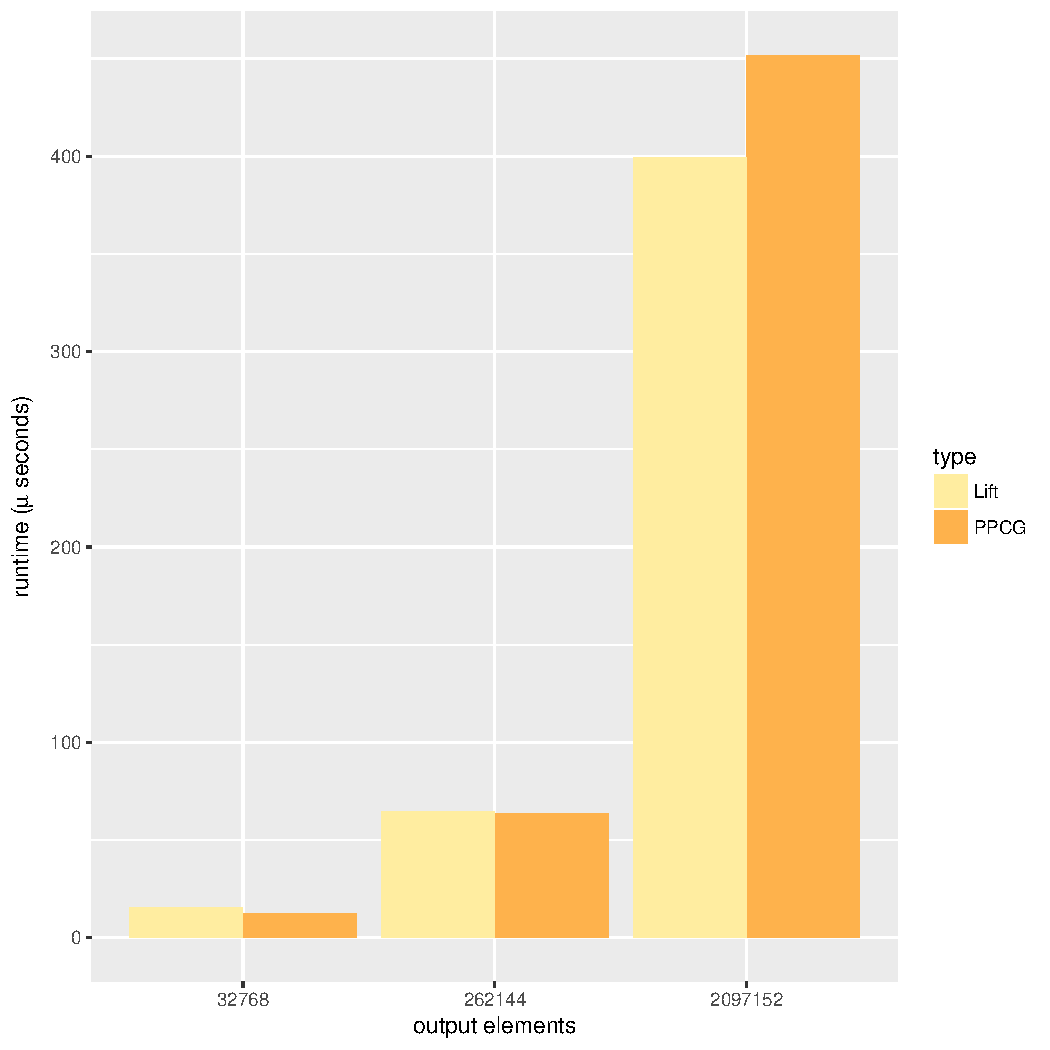
\includegraphics[scale=0.35]{img/plots/residual.pdf}
\end{frame}

\begin{frame}{Restrict}
	\center
	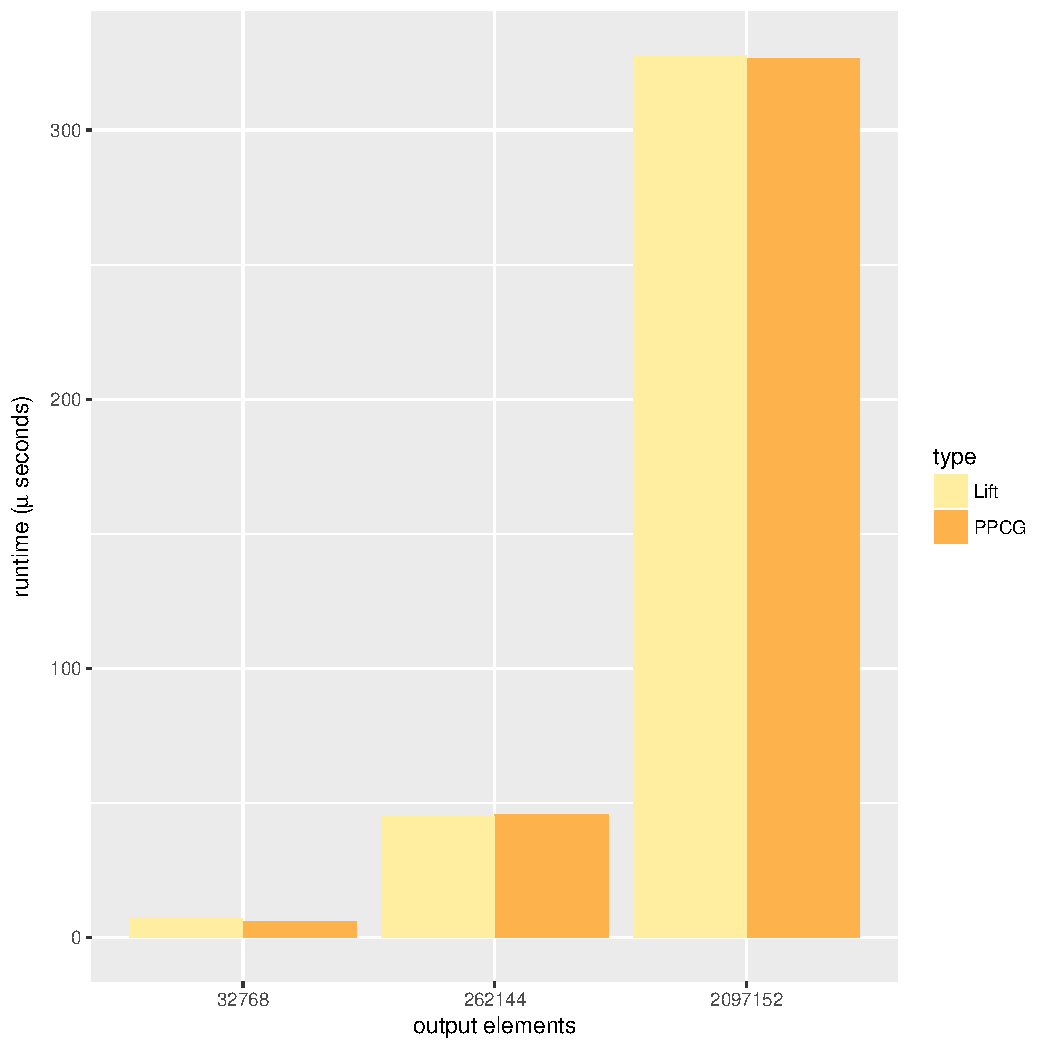
\includegraphics[scale=0.35]{img/plots/restrict.pdf}
\end{frame}

\begin{frame}{Interpolate}
	\center
	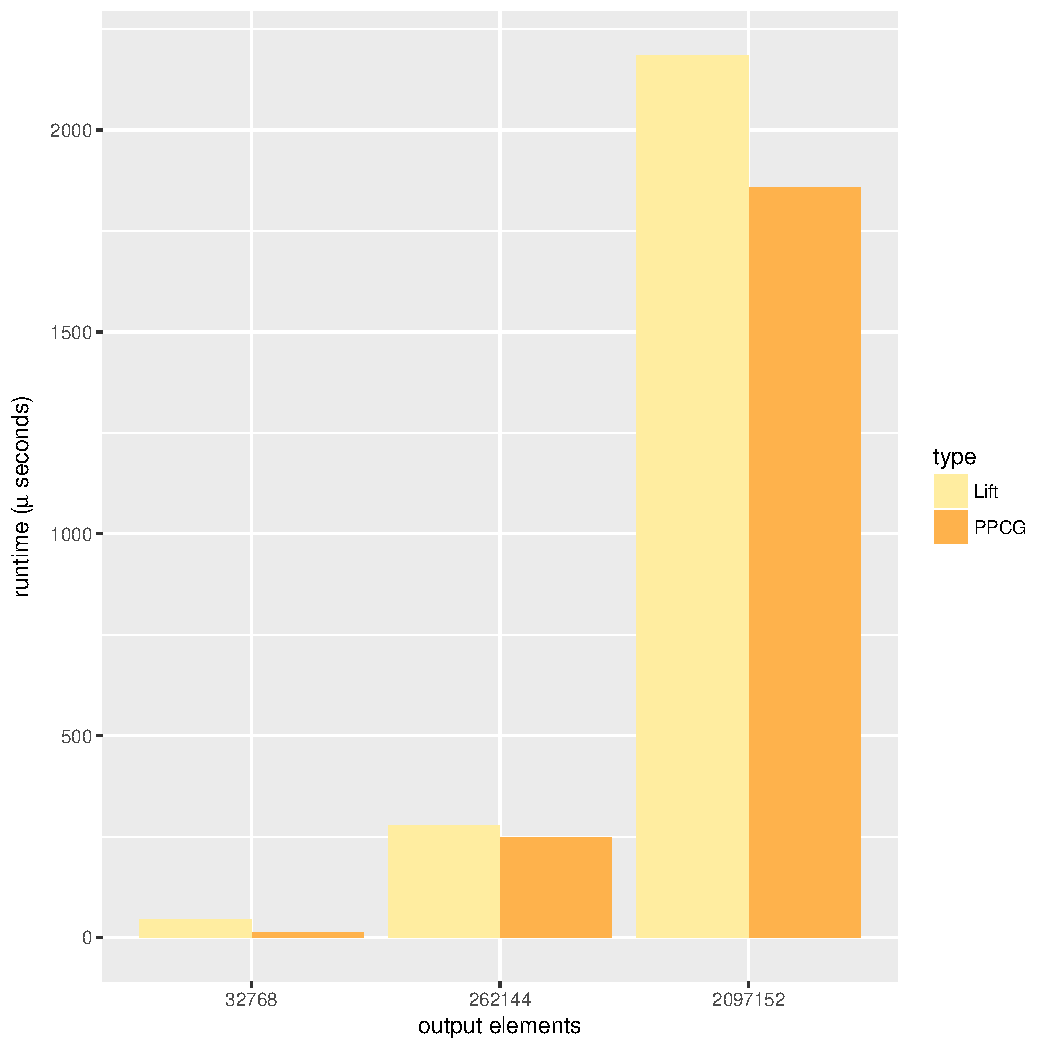
\includegraphics[scale=0.35]{img/plots/interpolate.pdf}
\end{frame}

\begin{frame}{Comparison}
	\center
	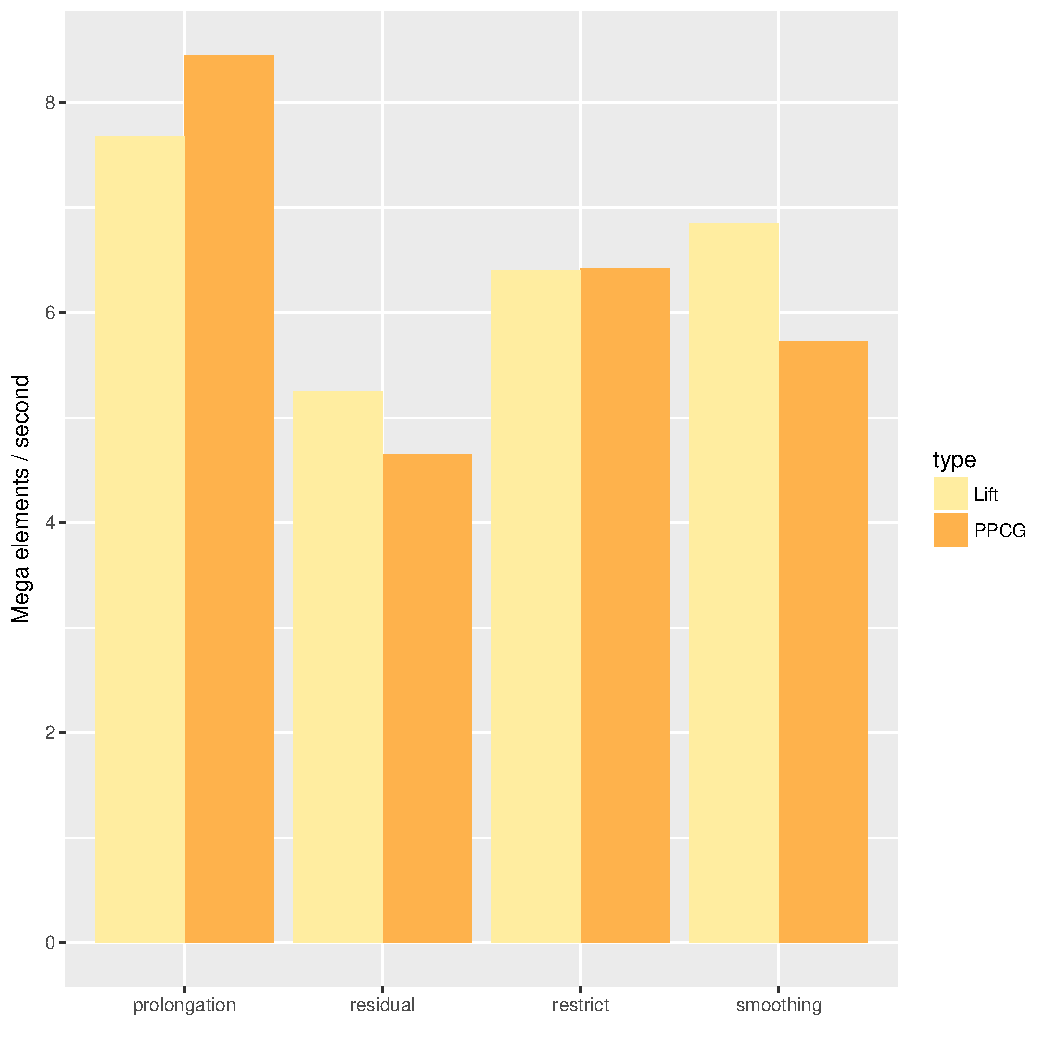
\includegraphics[scale=0.35]{img/plots/global.pdf}
\end{frame}



\end{document}
